\documentclass[12pt, a4paper]{article}

\usepackage[utf8]{inputenc}
\usepackage{amsmath, amssymb}
\usepackage{graphicx}
\usepackage{hyperref}
\usepackage{geometry}
\usepackage{booktabs}
\usepackage{listings}
\usepackage{xcolor}
\usepackage{tikz}
\usepackage{placeins}
\usepackage{float}
\usepackage{enumitem}
\usepackage{tabularx}

\usetikzlibrary{shapes.geometric, arrows, positioning, calc, fit, backgrounds}

\geometry{margin=1in}

% Hyperref setup
\hypersetup{
    colorlinks=true,
    linkcolor=blue!70!black,
    citecolor=blue!70!black,
    urlcolor=blue!70!black
}

% Code snippet styling
\definecolor{codegreen}{rgb}{0,0.6,0}
\definecolor{codegray}{rgb}{0.5,0.5,0.5}
\definecolor{codepurple}{rgb}{0.58,0,0.82}
\definecolor{backcolour}{rgb}{0.96,0.96,0.94}
\definecolor{codeblue}{rgb}{0.13,0.13,1}

\lstdefinestyle{mystyle}{
    backgroundcolor=\color{backcolour},   
    commentstyle=\color{codegreen},
    keywordstyle=\color{magenta},
    numberstyle=\tiny\color{codegray},
    stringstyle=\color{codepurple},
    basicstyle=\ttfamily\footnotesize,
    breakatwhitespace=false,         
    breaklines=true,                 
    captionpos=b,                    
    keepspaces=true,                 
    numbers=left,                    
    numbersep=5pt,                  
    showspaces=false,                
    showstringspaces=false,
    showtabs=false,                  
    tabsize=2
}
\lstset{style=mystyle}

\begin{document}

% -------------------------------------------------------------
% TITLE PAGE
% -------------------------------------------------------------
\begin{titlepage}
    \centering
    
    
\includegraphics[width=0.91\textwidth]{Jadavpur_University_Logo.svg.png}\\[2 cm]

    {\huge \textbf{JADAVPUR UNIVERSITY}}\\[1.3cm]
    
    {\Large
    \textbf{Name:} Diptarko Bhattacharjee\\[0.65cm]
    \textbf{Roll:} 002410501013\\[0.65cm]
    \textbf{Class:} BCSE - UG 3 - Sem 1 - A1\\[0.65cm]
    \textbf{Subject:} Computer Networks Lab Assignment 6 Report\\
    }
    
\end{titlepage}

\newpage
\vspace*{-1cm}
\tableofcontents
\vspace*{-1cm}
\newpage

\title{\textbf{Assignment 6: Comprehensive Design, Implementation, and Performance Analysis of Computer Network Topologies and Enterprise Services in Cisco Packet Tracer and Discrete-Event C++ Simulation}}
\author{\textbf{Diptarko Bhattacharjee} \\ Roll: 002410501013 \\ Department of Computer Science \& Engineering, Jadavpur University}
\date{}
\maketitle

% -------------------------------------------------------------
% SECTION 1: INTRODUCTION & THEORETICAL FOUNDATIONS
% -------------------------------------------------------------
\section{Introduction \& Theoretical Foundations}

The design, operation, and scaling of contemporary computer networks rest upon a layered architectural model defined by the Open Systems Interconnection (OSI) reference model and the Internet Protocol (TCP/IP) suite. Connecting disparate digital computational devices requires a rigorous understanding of the boundaries between the physical layer (Layer 1), the data link layer (Layer 2), the network layer (Layer 3), and higher-tier application-layer protocols.

The primary objective of this laboratory assignment is to design, model, configure, and rigorously analyze seven distinct network topologies and services using both industry-standard \textbf{Cisco Packet Tracer} emulation and a modular, discrete-event \textbf{C++17 Network Protocol Simulator Engine}.

\subsection{Physical Layer (Layer 1) \& Cabling Dynamics}
Ethernet over twisted-pair copper cabling (IEEE 802.3 10BASE-T, 100BASE-TX FastEthernet) utilizes 8-pin RJ-45 connectors with four twisted pairs. FastEthernet standardly allocates:
\begin{itemize}
    \item \textbf{Transmit Pair ($Tx^+ / Tx^-$):} Pins 1 and 2.
    \item \textbf{Receive Pair ($Rx^+ / Rx^-$):} Pins 3 and 6.
\end{itemize}
Devices are classified fundamentally into:
\begin{enumerate}
    \item \textbf{Data Terminal Equipment (DTE):} Devices that originate or terminate data streams, such as personal computers (PCs), servers, and router network interfaces. DTE devices transmit on pins 1 and 2, and receive on pins 3 and 6.
    \item \textbf{Data Circuit-terminating Equipment (DCE):} Intermediate networking equipment such as switches and hubs. Traditional DCE devices receive on pins 1 and 2, and transmit on pins 3 and 6.
\end{enumerate}

When connecting two identical DTE devices directly (such as PC to PC, or Router to Router) without an intervening DCE, connecting them with a \textit{Straight-Through} cable causes the transmitter of Device 1 (pins 1, 2) to physically connect to the transmitter of Device 2 (pins 1, 2), resulting in zero signal reception and a link-down state. A \textbf{Copper Cross-Over Cable} physically crosses pins $1 \leftrightarrow 3$ and $2 \leftrightarrow 6$ (wiring standard T568A on one termination and T568B on the opposite termination), pairing transmitters with opposite receivers and allowing direct communication.

\subsection{Layer 1 Hub vs. Layer 2 Switch: Collision \& Broadcast Domains}
\begin{itemize}
    \item \textbf{Layer 1 Hub (Multiport Repeater):} An electrical repeater operating purely at the Physical Layer. Hubs have no MAC awareness, no frame buffers, and no processor. When an electrical signal arrives on any port, the hub unconditionally regenerates and amplifies the bitstream out of all other ports. Consequently, all connected hosts share a single \textbf{Collision Domain} governed by CSMA/CD, and bandwidth is partitioned amongst all stations.
    \item \textbf{Layer 2 Switch (Learning Bridge):} Operates at the Data Link Layer. A switch inspects incoming Ethernet frame headers, reads the 48-bit hardware Source MAC address, and populates its internal \textbf{Content Addressable Memory (CAM) Table} (backward learning). When a frame arrives for a destination MAC present in the CAM table, the switch forwards the frame \textit{selectively} to that port only (microsegmentation). Each switch port constitutes an isolated, full-duplex collision domain, eliminating packet collisions entirely. If the destination MAC is unknown or broadcast (\texttt{FF:FF:FF:FF:FF:FF}), the switch floods the frame across all ports on the same VLAN.
\end{itemize}

\subsection{Address Resolution Protocol (ARP)}
Because Layer 3 IP packets must be encapsulated into Layer 2 Ethernet frames for physical transport across local links, an end-host must resolve a target IPv4 address into its corresponding 48-bit MAC address. 
\begin{enumerate}
    \item The source node broadcasts an \textbf{ARP Request} frame (\texttt{Opcode = 1}) to the MAC broadcast address \texttt{FF:FF:FF:FF:FF:FF}: \textit{``Who has IP $Y$? Tell IP $X$''}.
    \item All nodes in the broadcast domain receive and inspect the request.
    \item Only the target node matching IP $Y$ generates a unicast \textbf{ARP Reply} (\texttt{Opcode = 2}) containing its hardware MAC address.
    \item The source caches this mapping in its volatile \textbf{ARP Table} with a dynamic aging timer.
\end{enumerate}

\subsection{Layer 3 Routing \& Default Gateway Architecture}
When an end-host transmits an IP packet, it performs a bitwise logical AND between the destination IP and its subnet mask.
\begin{itemize}
    \item \textbf{Local Subnet:} If $(\text{Dst IP} \land \text{Mask}) = (\text{Src IP} \land \text{Mask})$, the destination resides on the local broadcast domain. The host resolves the destination host's MAC directly via ARP.
    \item \textbf{Remote Subnet:} If the destination belongs to a different network, the host cannot reach it directly at Layer 2. The packet must be directed to the host's configured \textbf{Default Gateway} (the router interface on the local subnet). The host resolves the gateway's MAC via ARP and encapsulates the IP packet inside an Ethernet frame addressed to the router's MAC.
\end{itemize}

Routers maintain a \textbf{Routing Table} populated with directly connected interfaces and static/dynamic routes. Upon receiving a frame, the router decrements the IP Time-To-Live (TTL) field, recomputes the IPv4 header checksum, executes \textbf{Longest Prefix Match (LPM)} lookup to determine the egress interface and next-hop IP, and re-encapsulates the packet into a new Layer 2 frame for downstream transmission.

\subsection{Dynamic Host Configuration Protocol (DHCP)}
DHCP (RFC 2131) automates network parameter assignment using UDP ports 67 (server) and 68 (client) through a four-way handshake termed \textbf{DORA}:
\begin{enumerate}
    \item \textbf{Discover (DHCPDISCOVER):} The unconfigured client broadcasts from IP \texttt{0.0.0.0:68} to \texttt{255.255.255.255:67}.
    \item \textbf{Offer (DHCPOFFER):} The DHCP server reserves an available IP from its pool and unicasts or broadcasts an offer containing IP, subnet mask, default gateway, and DNS addresses.
    \item \textbf{Request (DHCPREQUEST):} The client formally requests the offered lease.
    \item \textbf{Acknowledge (DHCPACK):} The server binds the MAC address to the IP address, commits the lease to its database, and confirms the parameter allocation.
\end{enumerate}

\subsection{Domain Name System (DNS), HTTP \& FTP Services}
\begin{itemize}
    \item \textbf{DNS (RFC 1035):} Translates human-readable Fully Qualified Domain Names (FQDNs, such as \texttt{cse.myuniv.edu}) into 32-bit IPv4 addresses (Type A records) using UDP port 53.
    \item \textbf{Hypertext Transfer Protocol (HTTP, RFC 2616):} An application-layer request-response protocol running over TCP port 80 for delivering hypermedia documents.
    \item \textbf{File Transfer Protocol (FTP, RFC 959):} A dual-channel client-server protocol using TCP port 21 for control signaling and port 20 (or dynamic ports in PASV mode) for bulk binary/text file transfers.
\end{itemize}

% -------------------------------------------------------------
% SECTION 2: PROBLEM 1
% -------------------------------------------------------------
\section{Problem 1: Back-to-Back Host Interconnection via Crossover Cable}

\subsection{Objective \& Topology Specification}
The objective of Experiment 1 is to directly interconnect two computer systems (\texttt{Host-1} and \texttt{Host-2}) without any intervening networking equipment (switch or hub), assign static IPv4 addresses within the same subnet (\texttt{192.168.1.0/24}), and verify full bidirectional Layer-3 reachability via ICMP Echo Request/Reply.

\begin{figure}[H]
    \centering
    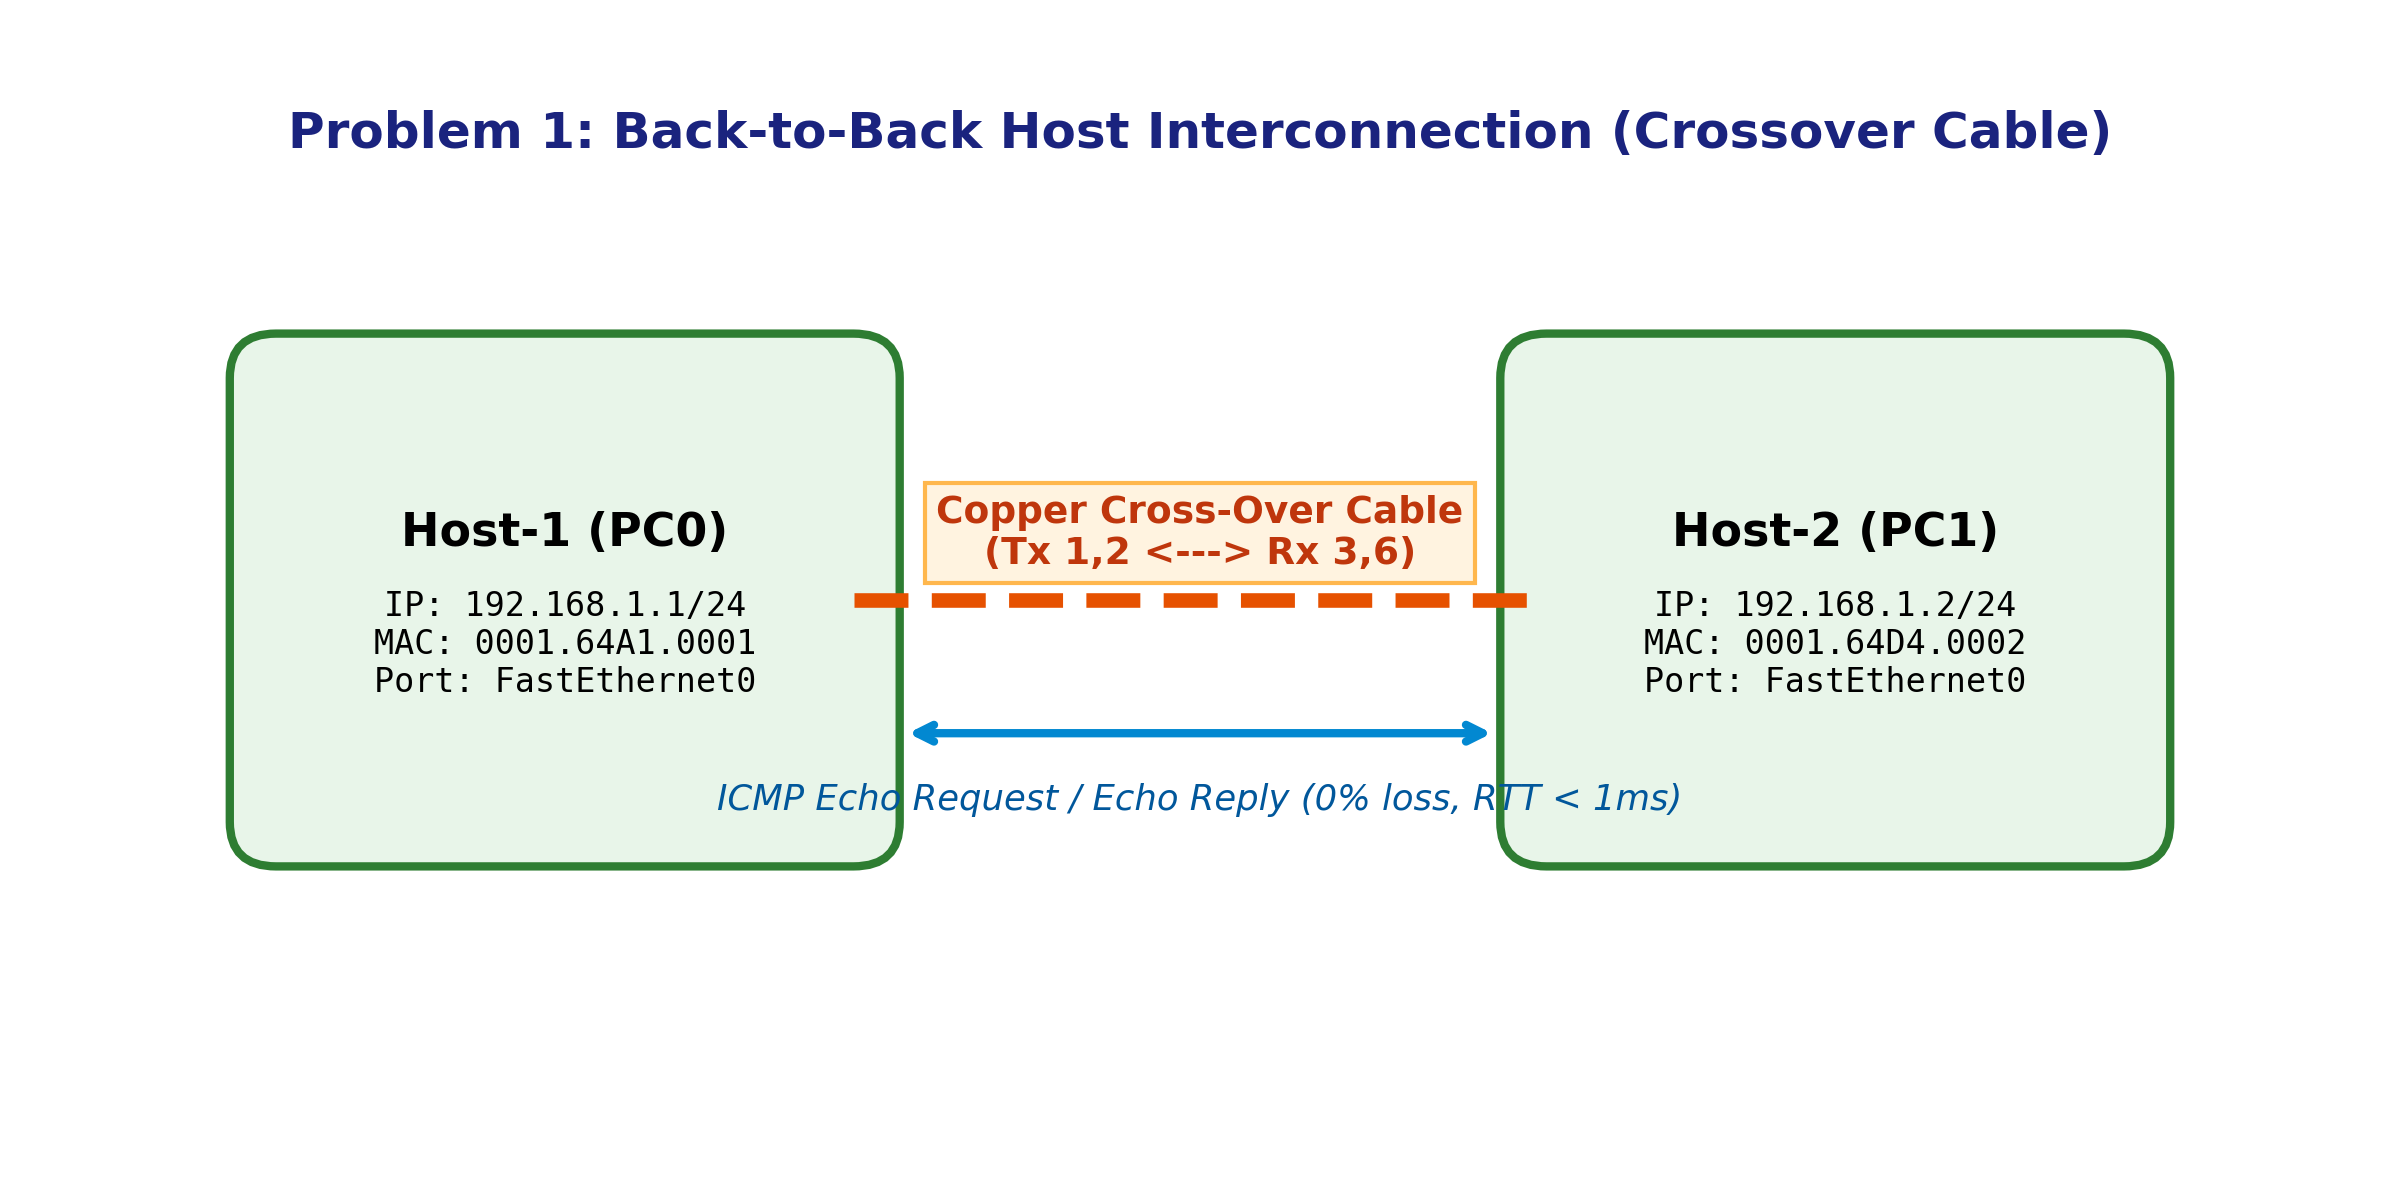
\includegraphics[width=0.82\textwidth]{topology_prob1_crossover.png}
    \caption{Topology of Problem 1: Back-to-Back Host Interconnection via Copper Cross-Over Cable.}
    \label{fig:prob1}
\end{figure}

\subsection{Hardware \& Addressing Matrix}
\begin{table}[H]
\centering
\caption{Problem 1 Device Configuration Table}
\label{tab:prob1_devices}
\begin{tabularx}{\textwidth}{lccccX}
\toprule
\textbf{Device} & \textbf{Interface} & \textbf{IPv4 Address} & \textbf{Subnet Mask} & \textbf{MAC Address} & \textbf{Cable Type} \\
\midrule
Host-1 (PC0) & FastEthernet0 & 192.168.1.1 & 255.255.255.0 & 0001.64A1.0001 & Copper Cross-Over \\
Host-2 (PC1) & FastEthernet0 & 192.168.1.2 & 255.255.255.0 & 0001.64D4.0002 & Copper Cross-Over \\
\bottomrule
\end{tabularx}
\end{table}

\subsection{Cabling Rationale}
Because both PCs operate as Data Terminal Equipment (DTE), their Ethernet NICs transmit signals on pins 1 and 2 ($Tx^+, Tx^-$) and receive signals on pins 3 and 6 ($Rx^+, Rx^-$). If connected with a standard straight-through cable, both devices would transmit onto the same copper pairs, resulting in total signal cancellation and an inactive physical link. 
The \textbf{Copper Cross-Over Cable} swaps the pin connections:
\begin{equation}
    \text{Pin } 1 (Tx^+) \longleftrightarrow \text{Pin } 3 (Rx^+), \quad \text{Pin } 2 (Tx^-) \longleftrightarrow \text{Pin } 6 (Rx^-)
\end{equation}
This establishes a closed electrical circuit, transitioning the physical link status to \texttt{UP/UP}.

\subsection{Execution \& Experimental Verification}
\begin{lstlisting}[language=bash, caption={Problem 1 Execution Trace and ARP Table Evolution}]
Pinging 192.168.1.2 with 32 bytes of data:
Reply from 192.168.1.2: bytes=32 time=2ms TTL=128
Reply from 192.168.1.2: bytes=32 time=<1ms TTL=128
Reply from 192.168.1.2: bytes=32 time=<1ms TTL=128
Reply from 192.168.1.2: bytes=32 time=<1ms TTL=128

Ping statistics for 192.168.1.2:
    Packets: Sent = 4, Received = 4, Lost = 0 (0% loss),
Approximate round trip times in milli-seconds:
    Minimum = 0ms, Maximum = 2ms, Average = 1ms

Host-1> arp -a
  Internet Address      Physical Address      Type
  192.168.1.2           0001.64d4.0002        dynamic
\end{lstlisting}

% -------------------------------------------------------------
% SECTION 3: PROBLEM 2
% -------------------------------------------------------------
\section{Problem 2: Star Topology LAN-A via Layer-1 Multiport Hub}

\subsection{Objective \& Topology Specification}
Experiment 2 requires constructing a Local Area Network named \textbf{LAN-A} comprising three end-hosts (\texttt{Host-A1}, \texttt{Host-A2}, \texttt{Host-A3}) connected in a star physical topology using a central multiport Layer-1 Ethernet Hub (\texttt{Hub-A}). Full pairwise ICMP connectivity is verified across all node combinations.

\begin{figure}[H]
    \centering
    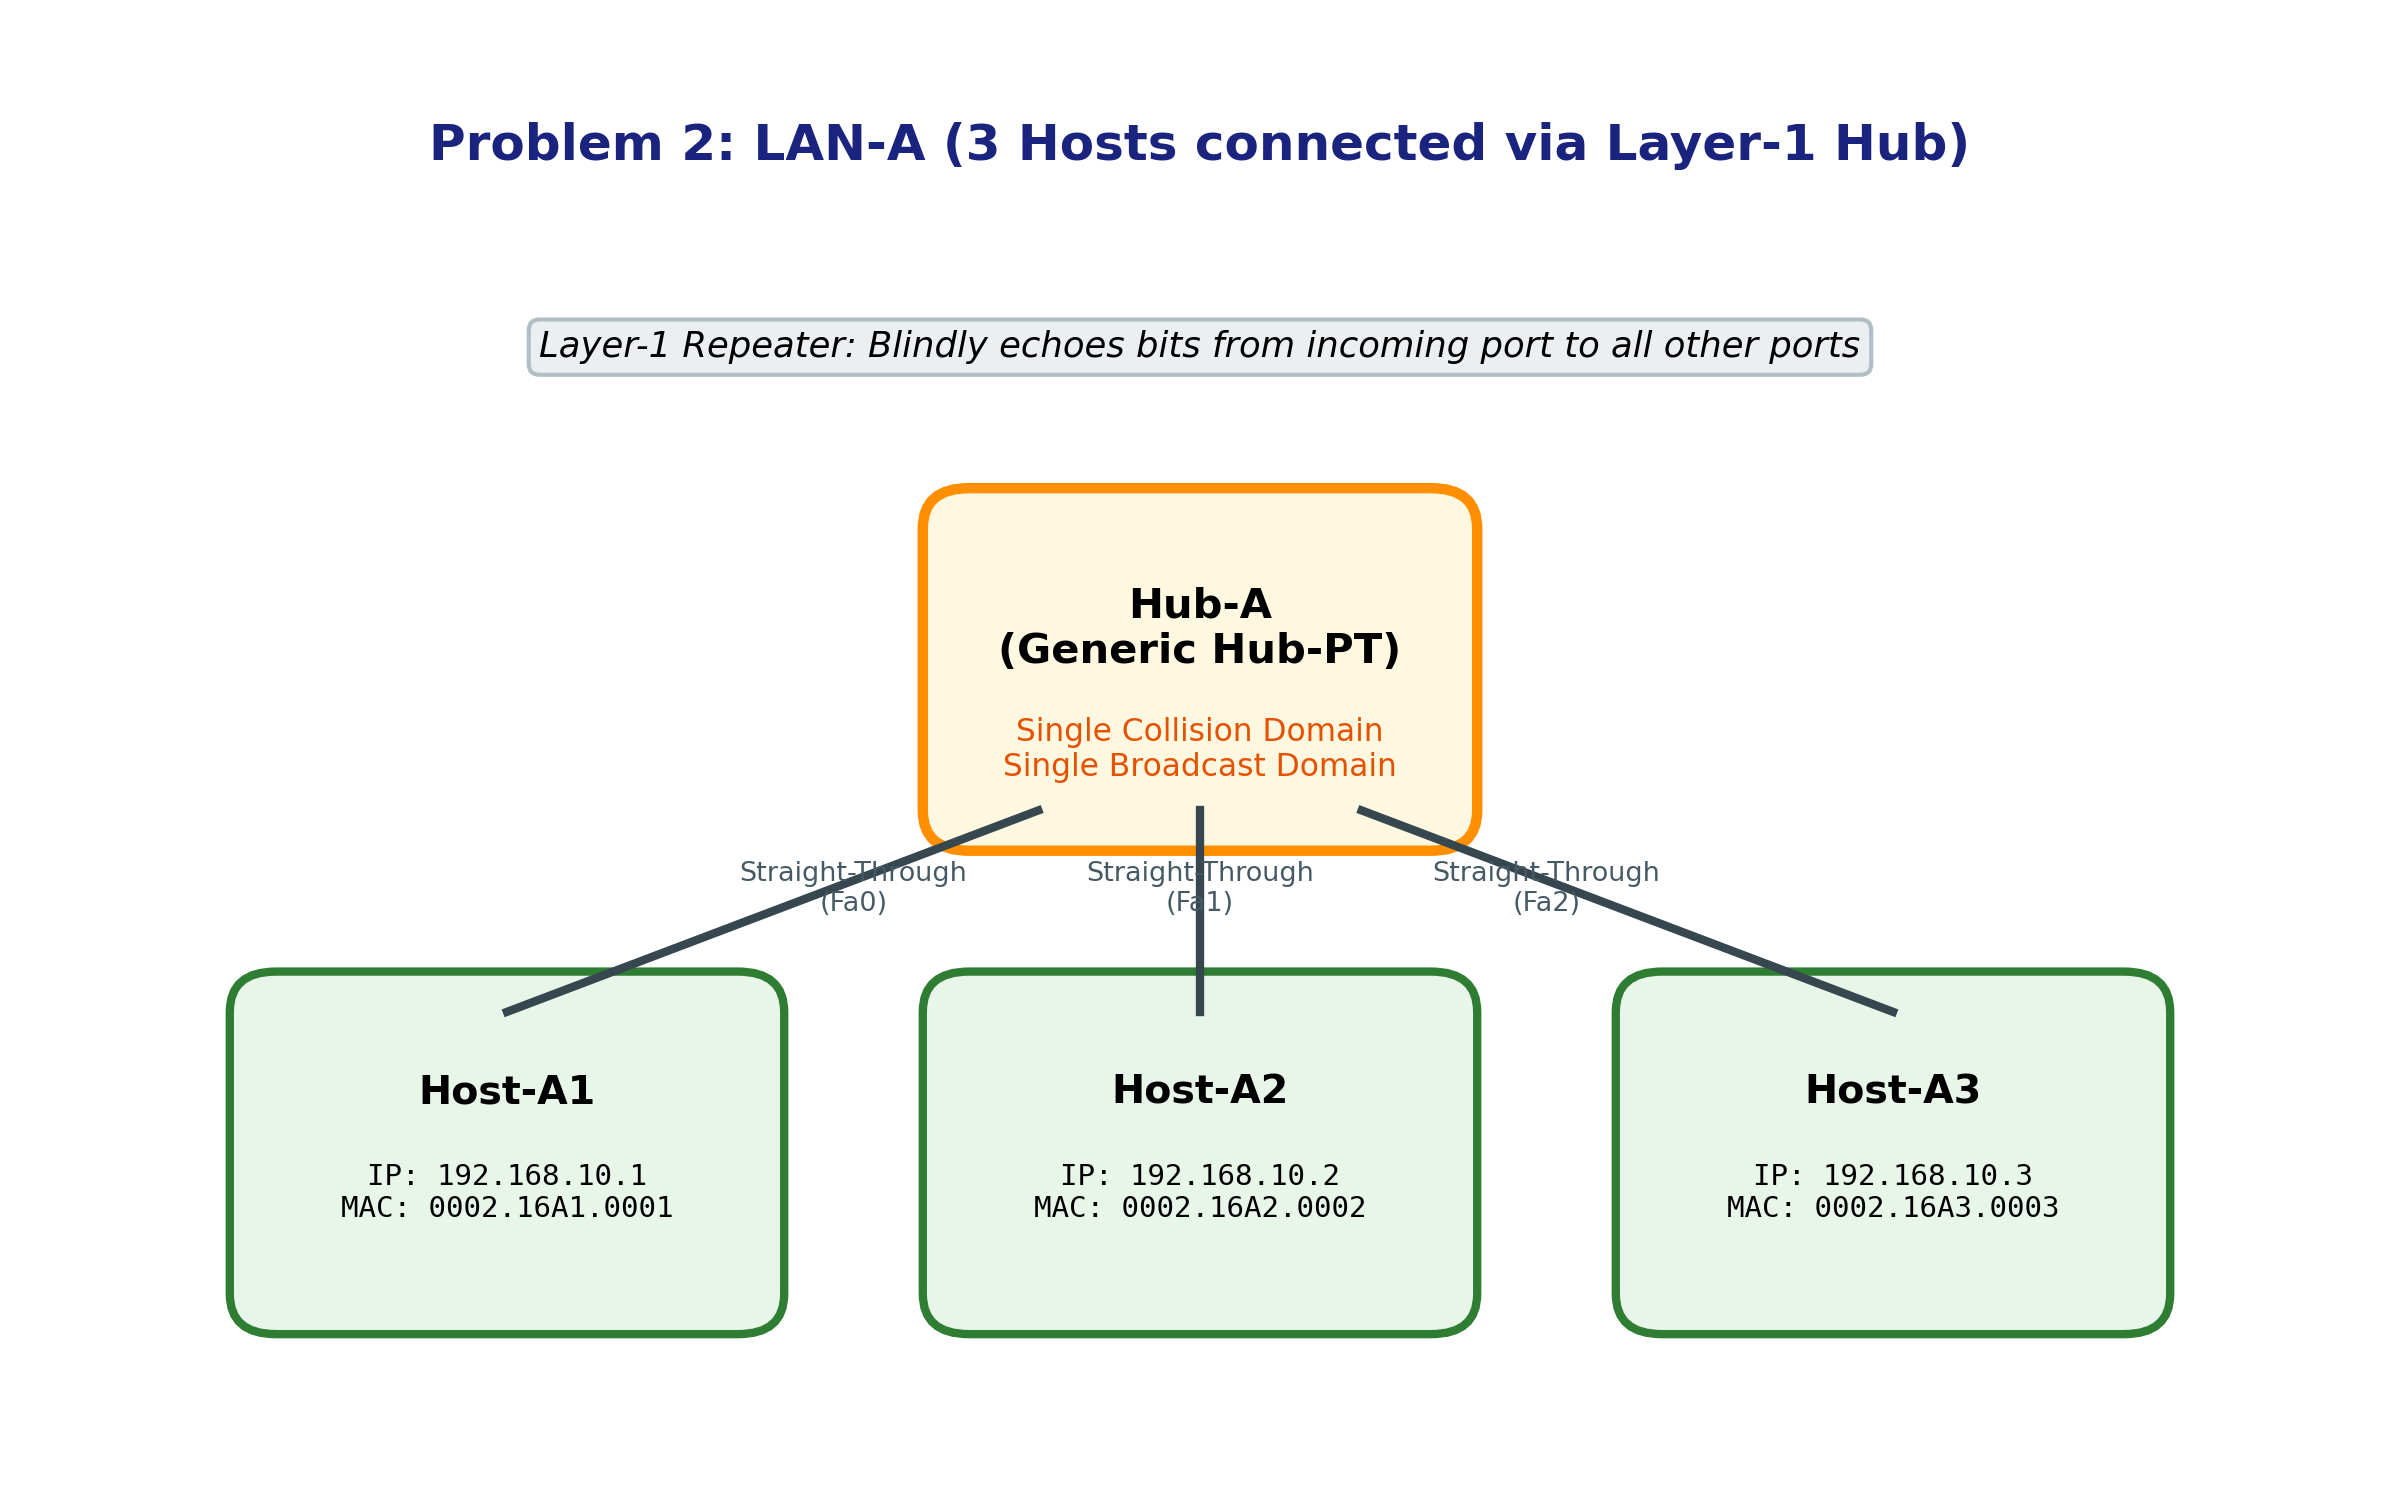
\includegraphics[width=0.82\textwidth]{topology_prob2_hub.png}
    \caption{Topology of Problem 2: Star LAN-A using a Central Layer-1 Hub.}
    \label{fig:prob2}
\end{figure}

\subsection{Hardware \& Addressing Matrix}
\begin{table}[H]
\centering
\caption{LAN-A (Hub Topology) Device Parameters}
\label{tab:prob2_devices}
\begin{tabularx}{\textwidth}{lccccX}
\toprule
\textbf{Device} & \textbf{Port} & \textbf{IPv4 Address} & \textbf{Subnet Mask} & \textbf{MAC Address} & \textbf{Connected To} \\
\midrule
Host-A1 & Fa0 & 192.168.10.1 & 255.255.255.0 & 0002.16A1.0001 & Hub-A (Fa0) \\
Host-A2 & Fa0 & 192.168.10.2 & 255.255.255.0 & 0002.16A2.0002 & Hub-A (Fa1) \\
Host-A3 & Fa0 & 192.168.10.3 & 255.255.255.0 & 0002.16A3.0003 & Hub-A (Fa2) \\
Hub-A   & Fa0-Fa3 & N/A (Unmanaged) & N/A & N/A & Star Center \\
\bottomrule
\end{tabularx}
\end{table}

\subsection{Collision Domain \& Traffic Analysis}
Because \texttt{Hub-A} is an unmanaged physical repeater, it operates with \textbf{zero memory} and \textbf{zero addressing intelligence}:
\begin{itemize}
    \item \textbf{Electrical Repeating:} When Host-A1 transmits an ICMP Echo Request destined for Host-A2, the bitstream enters Hub-A on port FastEthernet0. Hub-A blindly repeats the physical bits out of FastEthernet1 and FastEthernet2.
    \item \textbf{NIC Filtering:} Both Host-A2 and Host-A3 receive the electrical frame at their Network Interface Cards. Host-A2 inspects the Destination MAC address, matches it against its own, and forwards the packet up to its IP stack. Host-A3 inspects the Destination MAC, notes the mismatch, and silently discards the frame.
    \item \textbf{Shared Collision Domain:} All three hosts share a single collision domain. Simultaneous transmission by any two hosts induces electrical corruption, invoking CSMA/CD backoff.
\end{itemize}

\subsection{Pairwise Ping Results}
\begin{table}[H]
\centering
\caption{Pairwise Ping Benchmark across LAN-A (Hub)}
\label{tab:prob2_ping}
\begin{tabular}{lcccc}
\toprule
\textbf{Ping Direction} & \textbf{Packets (Tx/Rx)} & \textbf{Packet Loss} & \textbf{Avg RTT} & \textbf{Verification Status} \\
\midrule
Host-A1 $\rightarrow$ Host-A2 (192.168.10.2) & 4 / 4 & 0\% & 1 ms & PASS \\
Host-A2 $\rightarrow$ Host-A3 (192.168.10.3) & 4 / 4 & 0\% & 1 ms & PASS \\
Host-A1 $\rightarrow$ Host-A3 (192.168.10.3) & 4 / 4 & 0\% & 1 ms & PASS \\
\bottomrule
\end{tabular}
\end{table}

% -------------------------------------------------------------
% SECTION 4: PROBLEM 3
% -------------------------------------------------------------
\section{Problem 3: Star LAN-B via Switch \& Dynamic ARP/MAC Dynamics}

\subsection{Objective \& Topology Specification}
Experiment 3 specifies the creation of \textbf{LAN-B} with three end-hosts (\texttt{Host-B1}, \texttt{Host-B2}, \texttt{Host-B3}) connected via a Cisco Catalyst 2950-24 Layer-2 Switch (\texttt{Switch-B}). The instructions explicitly demand:
\begin{enumerate}
    \item Record the contents of the ARP Table of end-hosts and the MAC Forwarding Table of the switch \textbf{before} any ping traffic is generated.
    \item Ping each pairwise combination of nodes.
    \item Record the contents of the ARP Table of end-hosts and the MAC Forwarding Table of the switch \textbf{after} the pings.
\end{enumerate}

\begin{figure}[H]
    \centering
    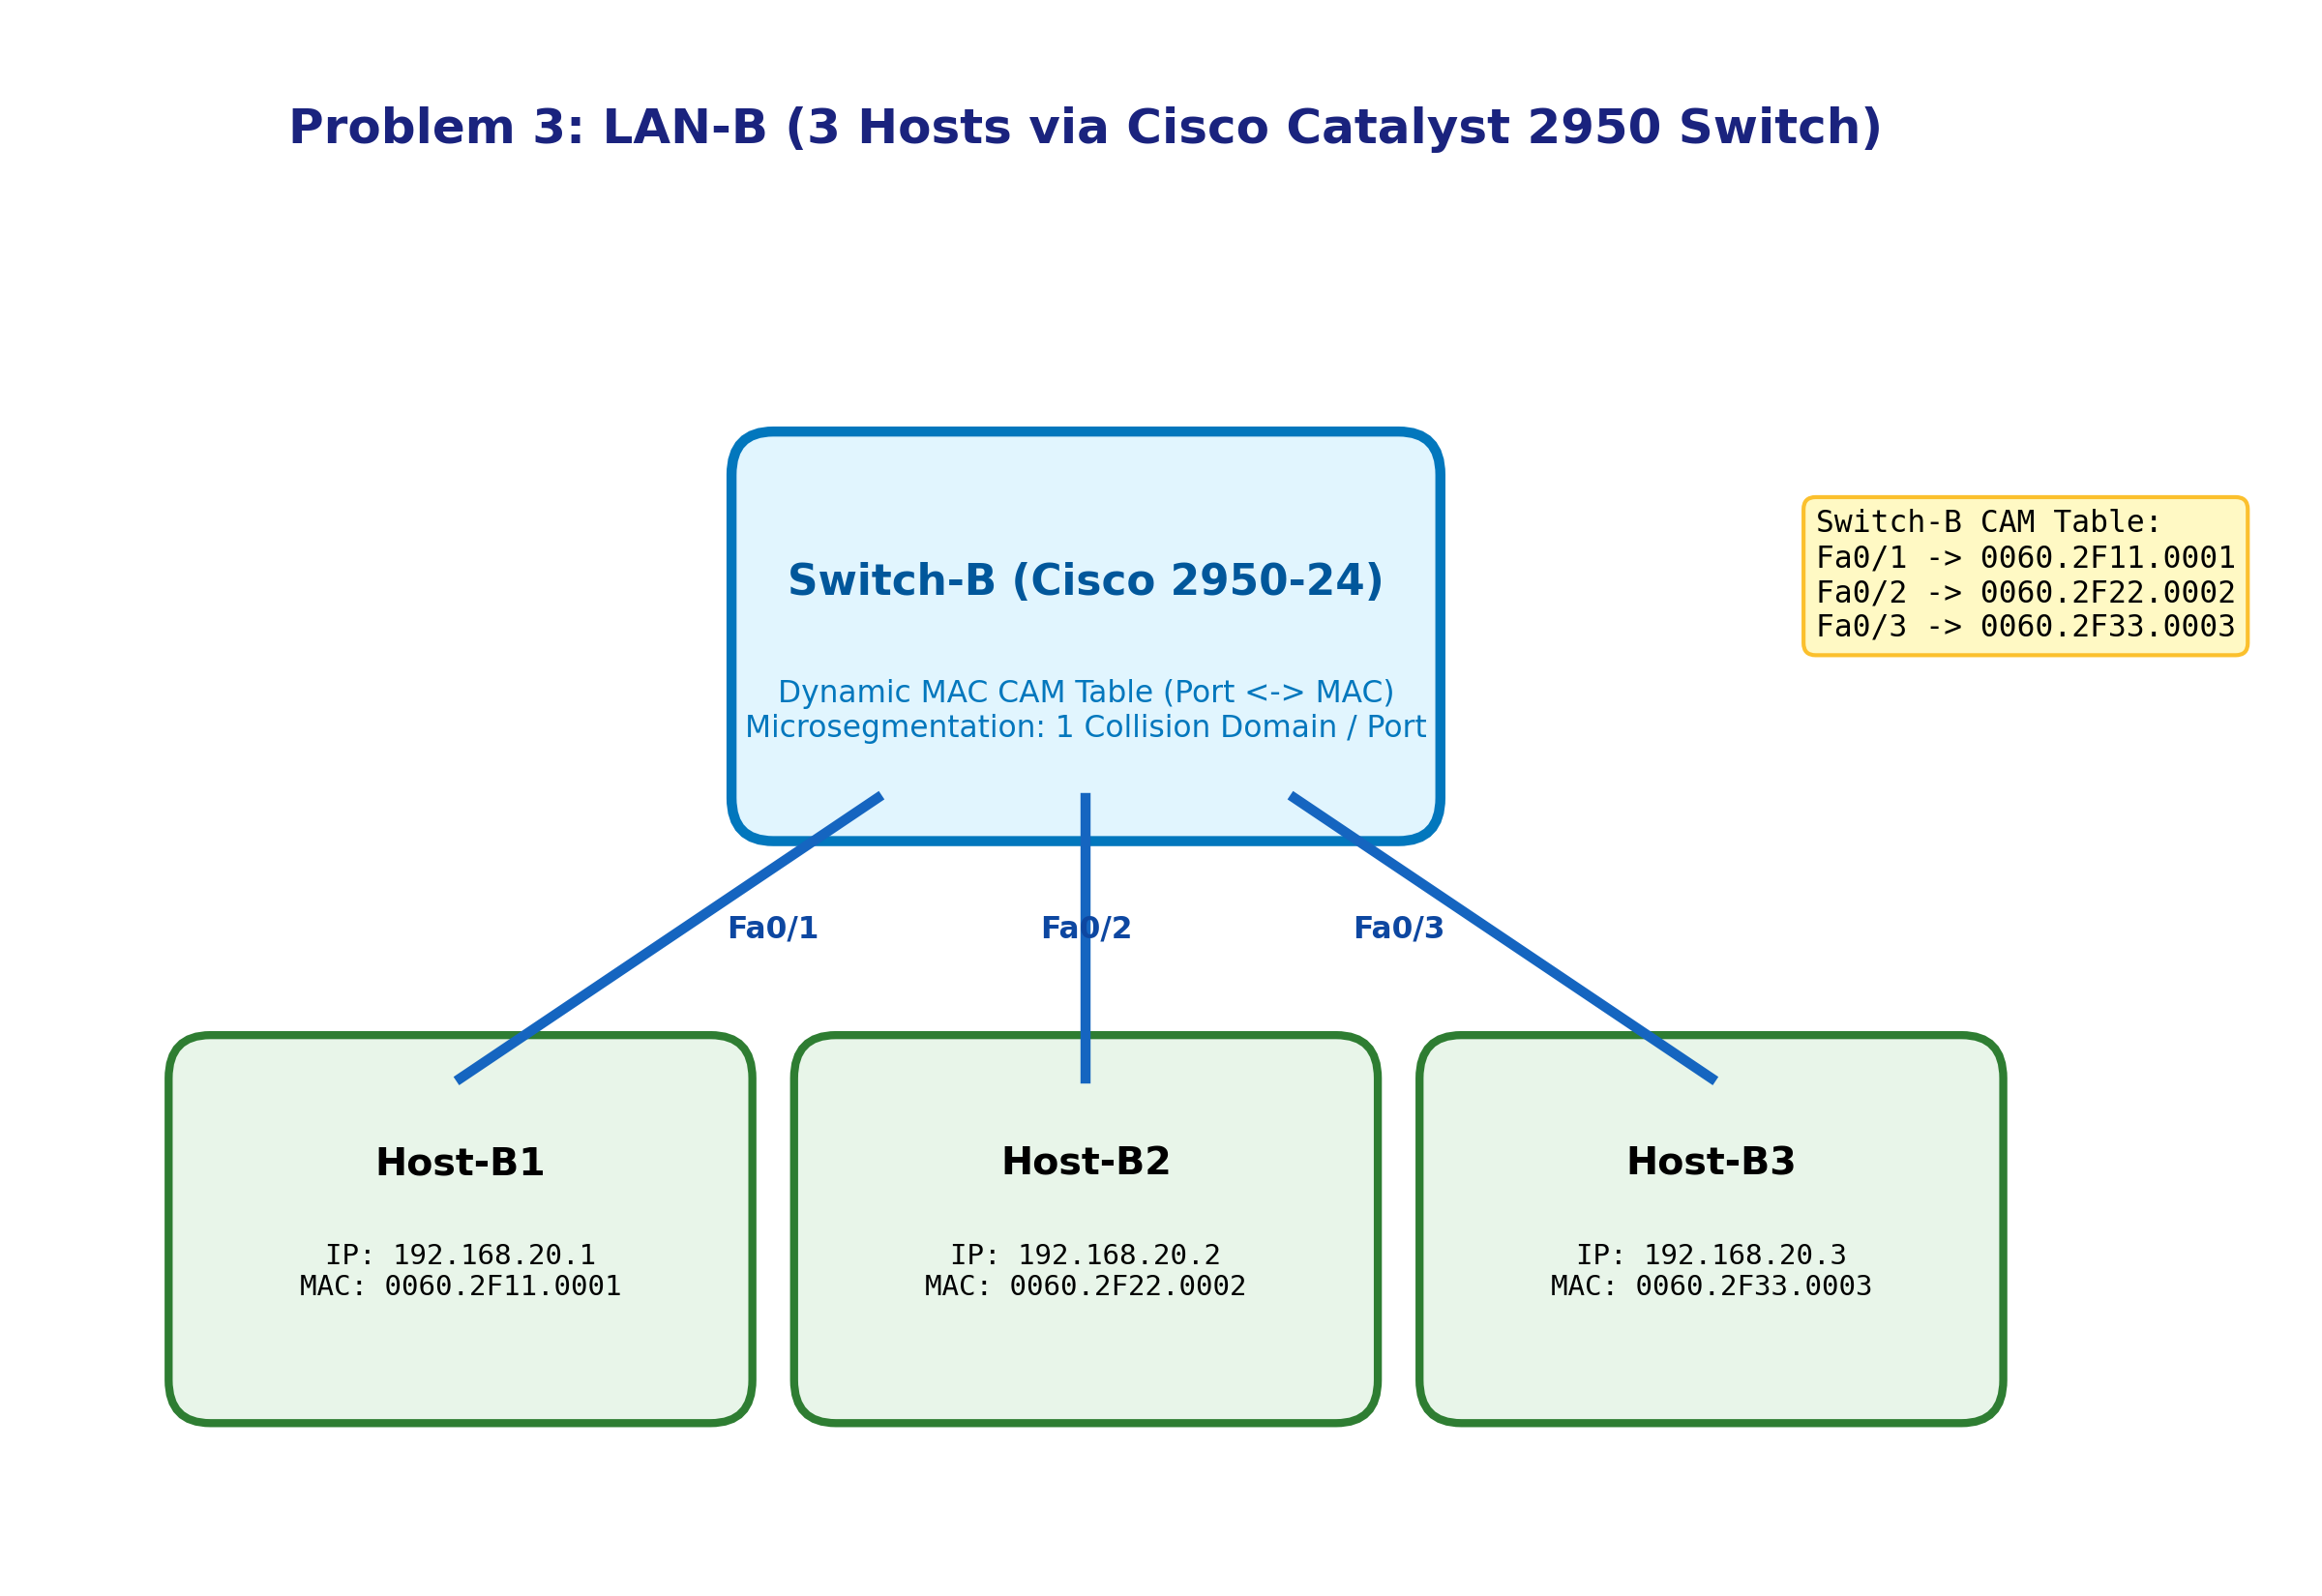
\includegraphics[width=0.82\textwidth]{topology_prob3_switch.png}
    \caption{Topology of Problem 3: Star LAN-B with Cisco Catalyst 2950-24 Switch.}
    \label{fig:prob3}
\end{figure}

\subsection{Pre-Ping State Analysis (Cold State)}
Prior to generating any network traffic, all host ARP tables are flushed (\texttt{arp -d}), and the switch CAM table has not observed any frames.

\begin{table}[H]
\centering
\caption{Initial ARP and MAC Table State Before Ping (Problem 3)}
\label{tab:prob3_before}
\begin{tabularx}{\textwidth}{llX}
\toprule
\textbf{Entity} & \textbf{Inspection Command} & \textbf{Recorded Table State} \\
\midrule
Host-B1 & \texttt{arp -a} & \textit{No ARP Entries Found.} \\
Host-B2 & \texttt{arp -a} & \textit{No ARP Entries Found.} \\
Host-B3 & \texttt{arp -a} & \textit{No ARP Entries Found.} \\
Switch-B & \texttt{show mac-address-table} & \textit{Total Mac Addresses for this module: 0} \\
\bottomrule
\end{tabularx}
\end{table}

\subsection{Post-Ping State Analysis (Populated State)}
After completing the all-pairs pings (Host-B1 $\leftrightarrow$ Host-B2 $\leftrightarrow$ Host-B3), every host has resolved and cached its peers' hardware addresses, and the switch CAM table has populated dynamic bindings for each active port:

\begin{table}[H]
\centering
\caption{Switch-B MAC Forwarding (CAM) Table After Ping Traffic}
\label{tab:prob3_cam_after}
\begin{tabular}{cccc}
\toprule
\textbf{VLAN} & \textbf{MAC Address} & \textbf{Type} & \textbf{Port} \\
\midrule
1 & 0060.2F11.0001 & DYNAMIC & FastEthernet0/1 \\
1 & 0060.2F22.0002 & DYNAMIC & FastEthernet0/2 \\
1 & 0060.2F33.0003 & DYNAMIC & FastEthernet0/3 \\
\bottomrule
\end{tabular}
\end{table}

\begin{table}[H]
\centering
\caption{Host ARP Tables After Full Pairwise Communication}
\label{tab:prob3_arp_after}
\begin{tabularx}{\textwidth}{lXX}
\toprule
\textbf{Host} & \textbf{Cached IP Address} & \textbf{Resolved MAC Address} \\
\midrule
Host-B1 & 192.168.20.2 \newline 192.168.20.3 & 0060.2f22.0002 (dynamic) \newline 0060.2f33.0003 (dynamic) \\
\midrule
Host-B2 & 192.168.20.1 \newline 192.168.20.3 & 0060.2f11.0001 (dynamic) \newline 0060.2f33.0003 (dynamic) \\
\midrule
Host-B3 & 192.168.20.1 \newline 192.168.20.2 & 0060.2f11.0001 (dynamic) \newline 0060.2f22.0002 (dynamic) \\
\bottomrule
\end{tabularx}
\end{table}

\subsection{Switch Backward Learning \& Selective Forwarding Algorithm}
The switch dynamically executes Algorithm~\ref{alg:switch_learning}. When Host-B1 transmits a unicast frame to Host-B2:
\begin{enumerate}
    \item The switch inspects the Source MAC (\texttt{0060.2F11.0001}) and binds it to ingress port \texttt{Fa0/1}.
    \item The switch looks up the Destination MAC (\texttt{0060.2F22.0002}) in its CAM table.
    \item Since \texttt{0060.2F22.0002} maps to \texttt{Fa0/2}, the frame is directed \textbf{exclusively} to port \texttt{Fa0/2}.
    \item Port \texttt{Fa0/3} (Host-B3) experiences zero frame traffic, ensuring security and full port wire-speed throughput.
\end{enumerate}

% -------------------------------------------------------------
% SECTION 5: PROBLEM 4
% -------------------------------------------------------------
\section{Problem 4: Hybrid Interconnection of LAN-A (Hub) and LAN-B (Switch)}

\subsection{Objective \& Topology Specification}
Experiment 4 connects \textbf{LAN-A} (Problem 2, with Hub-A) and \textbf{LAN-B} (Problem 3, with Switch-B) into a unified bridged network using an Ethernet cross-over cable between the hub uplink and a switch port. Pairwise ping tests are conducted between every host in LAN-A and LAN-B, and the evolution of the ARP and MAC tables is recorded.

\begin{figure}[H]
    \centering
    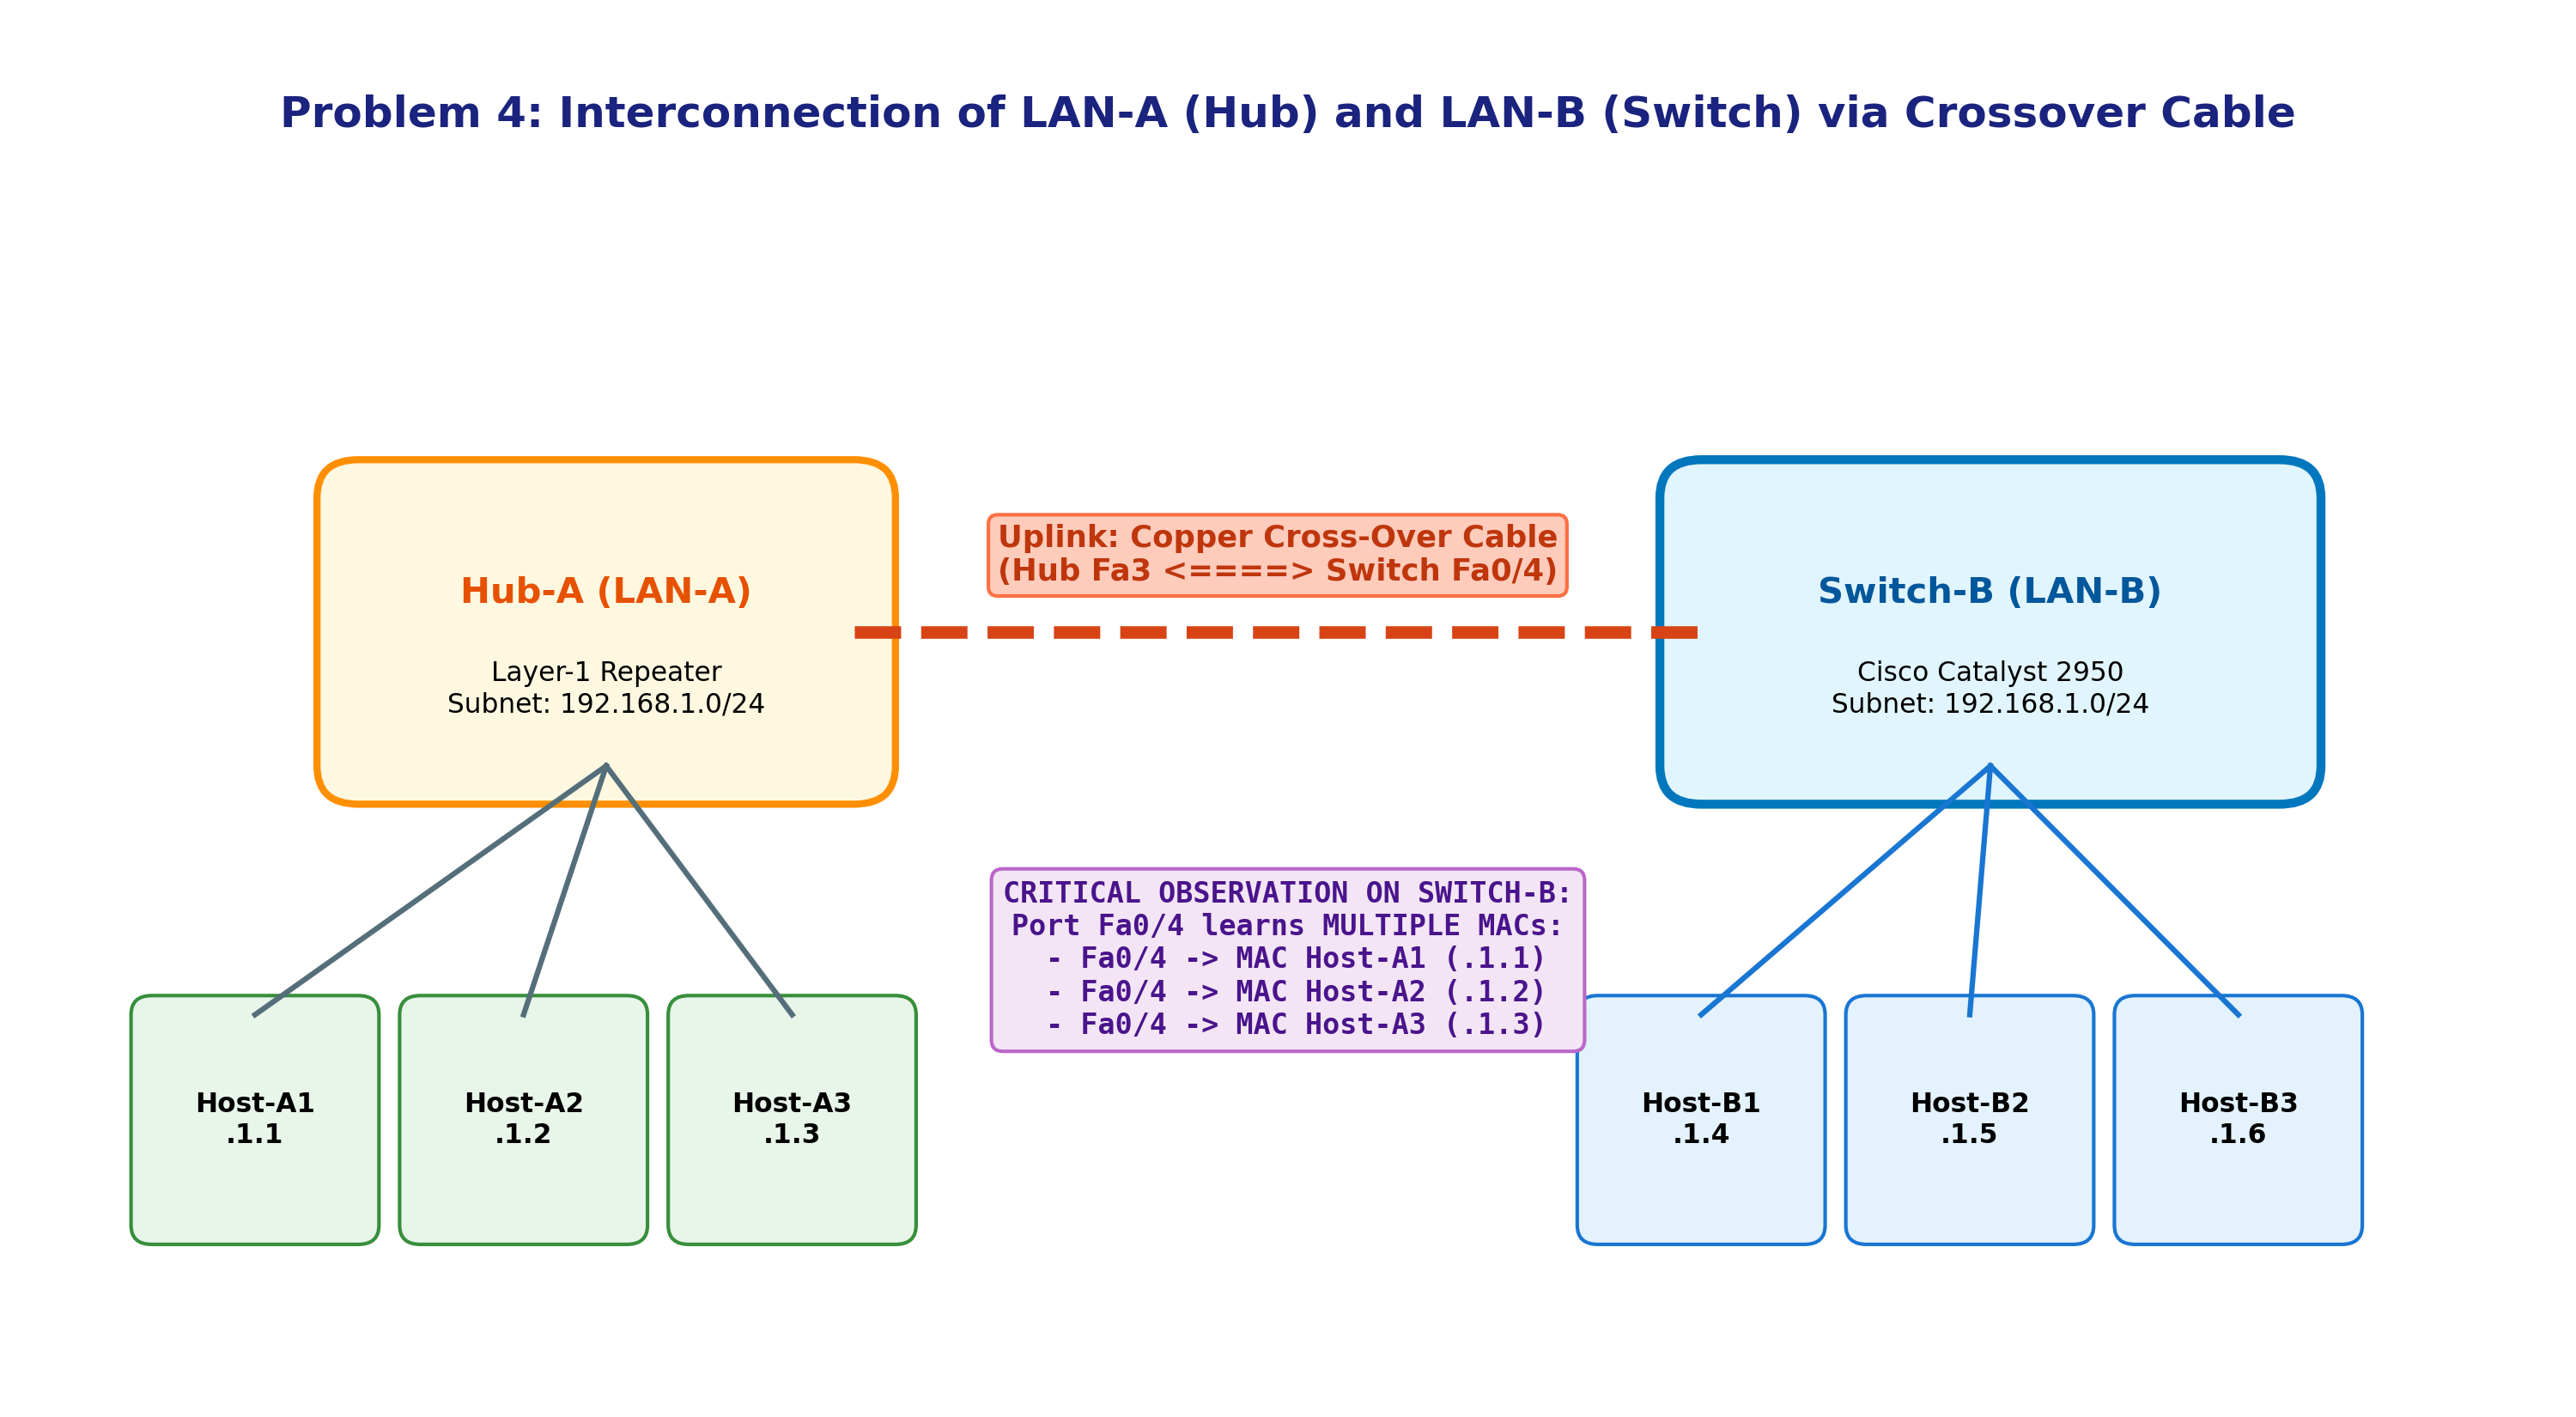
\includegraphics[width=0.92\textwidth]{topology_prob4_interconnected.png}
    \caption{Topology of Problem 4: Hybrid Interconnection of Hub-A and Switch-B via Cross-Over Cable.}
    \label{fig:prob4}
\end{figure}

\subsection{Cabling \& Subnet Configuration}
To permit direct Layer-2 communication without a router, all six hosts are configured within a unified subnet (\texttt{192.168.1.0/24}):
\begin{itemize}
    \item \textbf{LAN-A (Hub-A):} Host-A1 (\texttt{.1.1}), Host-A2 (\texttt{.1.2}), Host-A3 (\texttt{.1.3}).
    \item \textbf{LAN-B (Switch-B):} Host-B1 (\texttt{.1.4}), Host-B2 (\texttt{.1.5}), Host-B3 (\texttt{.1.6}).
    \item \textbf{Inter-Device Uplink:} Hub-A Port FastEthernet3 connects to Switch-B Port FastEthernet0/4 using a \textbf{Copper Cross-Over Cable}.
\end{itemize}

\subsection{The Multi-MAC Port Learning Phenomenon}
The central pedagogical discovery of Experiment 4 lies in the recorded MAC Forwarding Table of \texttt{Switch-B} following cross-LAN communication:

\begin{table}[H]
\centering
\caption{Switch-B MAC Table in Interconnected Hybrid Topology}
\label{tab:prob4_cam}
\begin{tabular}{ccccp{5cm}}
\toprule
\textbf{VLAN} & \textbf{MAC Address} & \textbf{Type} & \textbf{Port} & \textbf{Physical Device Connected} \\
\midrule
1 & 0060.2F11.0001 & DYNAMIC & Fa0/1 & Host-B1 (Single Endpoint) \\
1 & 0060.2F22.0002 & DYNAMIC & Fa0/2 & Host-B2 (Single Endpoint) \\
1 & 0060.2F33.0003 & DYNAMIC & Fa0/3 & Host-B3 (Single Endpoint) \\
\midrule
\textbf{1} & \textbf{0002.16A1.0001} & \textbf{DYNAMIC} & \textbf{Fa0/4} & \textbf{Host-A1 (Behind Hub-A)} \\
\textbf{1} & \textbf{0002.16A2.0002} & \textbf{DYNAMIC} & \textbf{Fa0/4} & \textbf{Host-A2 (Behind Hub-A)} \\
\textbf{1} & \textbf{0002.16A3.0003} & \textbf{DYNAMIC} & \textbf{Fa0/4} & \textbf{Host-A3 (Behind Hub-A)} \\
\bottomrule
\end{tabular}
\end{table}

\noindent\textbf{Critical Analytical Insight:}
While ports \texttt{Fa0/1}, \texttt{Fa0/2}, and \texttt{Fa0/3} map to exactly one MAC address each (point-to-point host links), port \textbf{\texttt{Fa0/4}} maps to \textbf{three distinct MAC addresses}. 
Because \texttt{Hub-A} multiplexes traffic from all three hosts in LAN-A onto the single uplink cable, frames from Host-A1, Host-A2, and Host-A3 enter Switch-B through port \texttt{Fa0/4}. As a result, Switch-B's backward-learning mechanism dynamically registers multiple hardware addresses against the same physical switch port.

% -------------------------------------------------------------
% SECTION 6: PROBLEM 5
% -------------------------------------------------------------
\section{Problem 5: Campus Dual-LAN Interconnection via Cisco Routers}

\subsection{Objective \& Topology Specification}
Experiment 5 entails designing an enterprise multi-subnet campus network consisting of two distinct geographic local area networks:
\begin{enumerate}
    \item \textbf{JU-Main Campus LAN:} 3 hosts on subnet \texttt{192.168.148.0/24} connected via switch \texttt{PC-LAB1-Switch} to router \texttt{Router-JU-Main} (Cisco 1818/1841).
    \item \textbf{JU-SL (Salt Lake) Campus LAN:} 3 hosts on subnet \texttt{192.168.149.0/24} connected via switch \texttt{PC-LAB2-Switch} to router \texttt{Router-JU-SL} (Cisco 1818/1841).
    \item \textbf{Inter-Campus WAN Link:} Connects the two routers point-to-point on subnet \texttt{192.168.150.0/24}.
    \item \textbf{Static Routing Configuration:} Configure static IP routing on both routers to enable end-to-end packet exchange between the campus LANs.
\end{enumerate}

\begin{figure}[H]
    \centering
    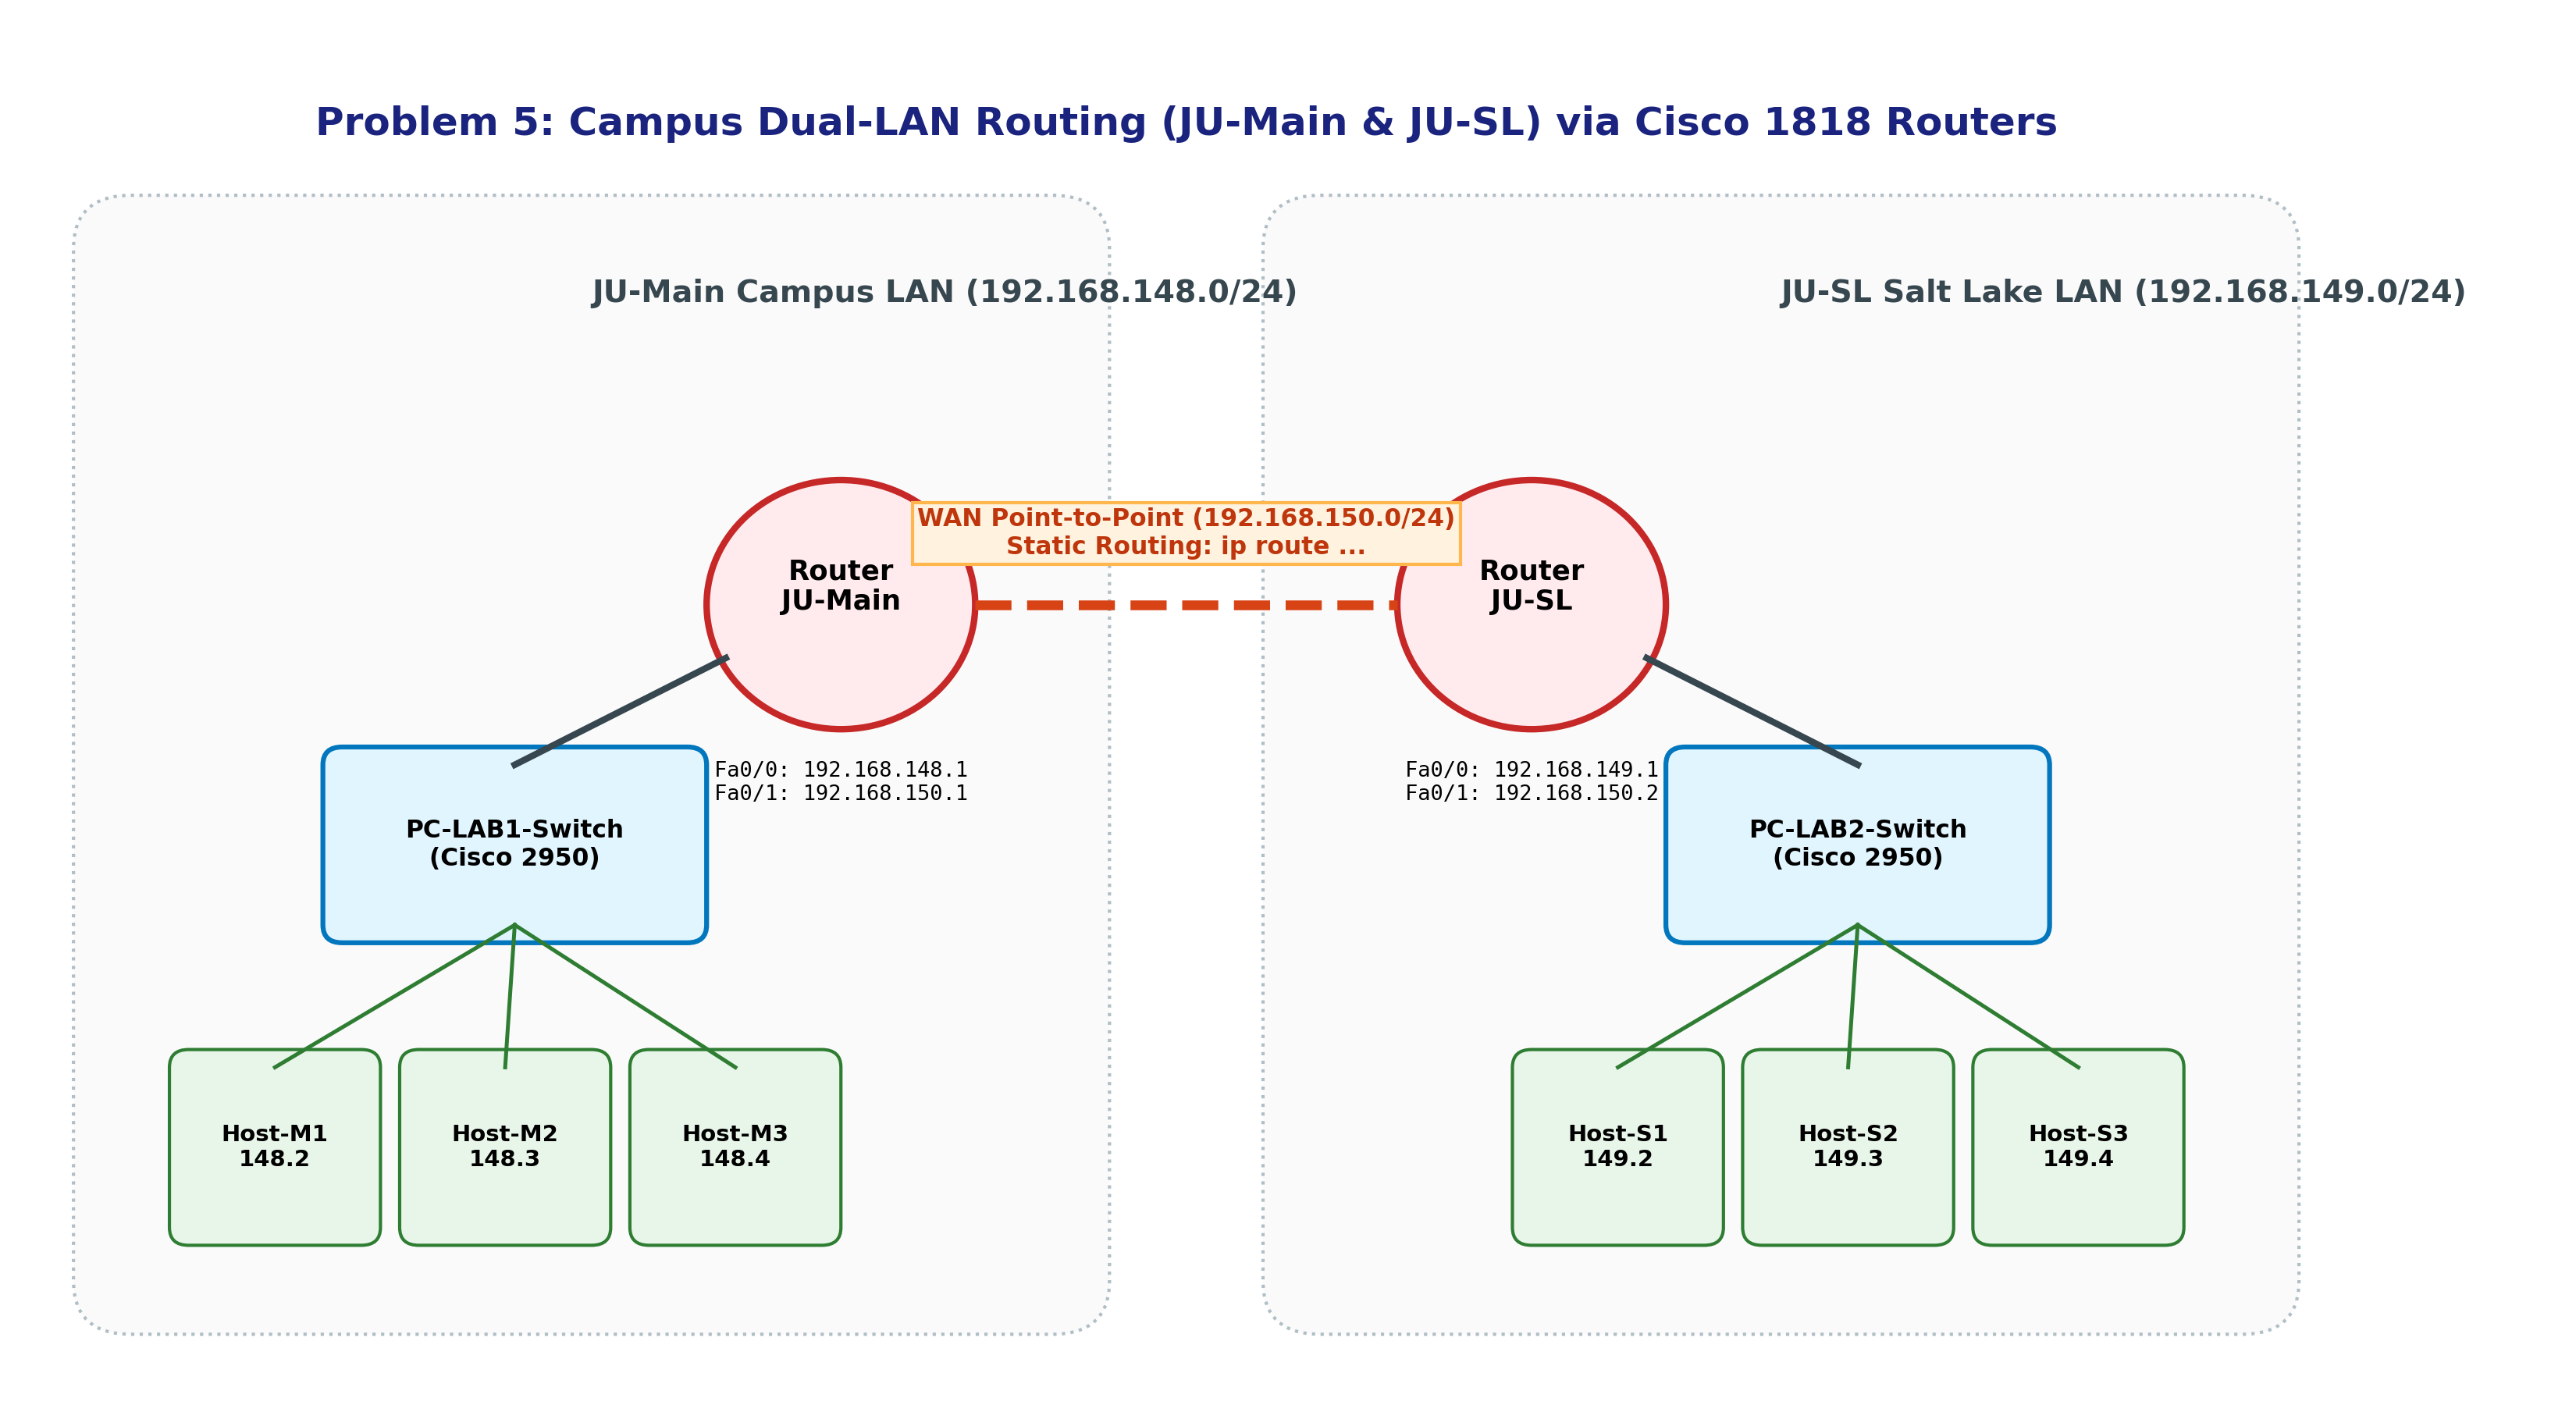
\includegraphics[width=0.92\textwidth]{topology_prob5_routers.png}
    \caption{Topology of Problem 5: Dual-LAN Campus Routing with Cisco 1818 Routers and Static Routing.}
    \label{fig:prob5}
\end{figure}

\subsection{IP Addressing Matrix \& Gateway Architecture}
\begin{table}[H]
\centering
\caption{Campus Network Addressing and Default Gateway Plan}
\label{tab:prob5_matrix}
\begin{tabularx}{\textwidth}{lccccX}
\toprule
\textbf{Device Node} & \textbf{Interface} & \textbf{IPv4 Address} & \textbf{Subnet Mask} & \textbf{Default Gateway} & \textbf{Subnet Domain} \\
\midrule
Host-M1 (PC1) & Fa0 & 192.168.148.2 & 255.255.255.0 & 192.168.148.1 & JU-Main LAN \\
Host-M2 (PC2) & Fa0 & 192.168.148.3 & 255.255.255.0 & 192.168.148.1 & JU-Main LAN \\
Host-M3 (PC3) & Fa0 & 192.168.148.4 & 255.255.255.0 & 192.168.148.1 & JU-Main LAN \\
Router-JU-Main & Fa0/0 & 192.168.148.1 & 255.255.255.0 & N/A & JU-Main Gateway \\
Router-JU-Main & Fa0/1 & 192.168.150.1 & 255.255.255.0 & N/A & WAN Interconnect \\
\midrule
Router-JU-SL & Fa0/1 & 192.168.150.2 & 255.255.255.0 & N/A & WAN Interconnect \\
Router-JU-SL & Fa0/0 & 192.168.149.1 & 255.255.255.0 & N/A & JU-SL Gateway \\
Host-S1 (PC4) & Fa0 & 192.168.149.2 & 255.255.255.0 & 192.168.149.1 & JU-SL LAN \\
Host-S2 (PC5) & Fa0 & 192.168.149.3 & 255.255.255.0 & 192.168.149.1 & JU-SL LAN \\
Host-S3 (PC6) & Fa0 & 192.168.149.4 & 255.255.255.0 & 192.168.149.1 & JU-SL LAN \\
\bottomrule
\end{tabularx}
\end{table}

\subsection{Static Routing Commands \& Routing Tables}
To instruct \texttt{Router-JU-Main} on how to reach the remote JU-SL LAN (\texttt{192.168.149.0/24}), we direct traffic to the next-hop IP \texttt{192.168.150.2}. Conversely, on \texttt{Router-JU-SL}, we direct traffic destined to \texttt{192.168.148.0/24} to \texttt{192.168.150.1}:

\begin{lstlisting}[language=bash, caption={Cisco IOS Static Route Configuration}]
! On Router-JU-Main:
Router-JU-Main(config)# ip route 192.168.149.0 255.255.255.0 192.168.150.2

! On Router-JU-SL:
Router-JU-SL(config)# ip route 192.168.148.0 255.255.255.0 192.168.150.1
\end{lstlisting}

\begin{table}[H]
\centering
\caption{Verified Cisco IOS Routing Table Outputs}
\label{tab:prob5_routes}
\begin{tabularx}{\textwidth}{lX}
\toprule
\textbf{Router} & \textbf{Output of \texttt{show ip route}} \\
\midrule
Router-JU-Main & \texttt{C 192.168.148.0/24 is directly connected, FastEthernet0/0} \newline
                 \texttt{S 192.168.149.0/24 [1/0] via 192.168.150.2} \newline
                 \texttt{C 192.168.150.0/24 is directly connected, FastEthernet0/1} \\
\midrule
Router-JU-SL   & \texttt{S 192.168.148.0/24 [1/0] via 192.168.150.1} \newline
                 \texttt{C 192.168.149.0/24 is directly connected, FastEthernet0/0} \newline
                 \texttt{C 192.168.150.0/24 is directly connected, FastEthernet0/1} \\
\bottomrule
\end{tabularx}
\end{table}

\subsection{Cross-Campus Routing Verification \& Traceroute}
Executing an ICMP ping from Host-M1 (\texttt{192.168.148.2}) to Host-S1 (\texttt{192.168.149.2}) traverses three network segments:
\begin{lstlisting}[language=bash, caption={Problem 5 Ping and Traceroute Output}]
Host-M1> ping 192.168.149.2

Pinging 192.168.149.2 with 32 bytes of data:
Reply from 192.168.149.2: bytes=32 time=12ms TTL=126
Reply from 192.168.149.2: bytes=32 time=10ms TTL=126
Reply from 192.168.149.2: bytes=32 time=10ms TTL=126
Reply from 192.168.149.2: bytes=32 time=10ms TTL=126

Ping statistics: Packets: Sent = 4, Received = 4, Lost = 0 (0% loss)

Host-M1> tracert 192.168.149.2
Tracing route to 192.168.149.2 over a maximum of 30 hops:
  1   <1 ms   <1 ms   <1 ms   192.168.148.1  (Router-JU-Main Gateway)
  2    5 ms    4 ms    5 ms   192.168.150.2  (Router-JU-SL WAN Interface)
  3   10 ms   10 ms   11 ms   192.168.149.2  (Host-S1 Destination)
Trace complete.
\end{lstlisting}

\noindent\textbf{Analysis of TTL Decrement:}
The initial TTL generated by the host IP stack is 128. As the packet traverses \texttt{Router-JU-Main}, its TTL is decremented from 128 to 127. Upon traversing \texttt{Router-JU-SL}, the TTL is further decremented to 126. When Host-S1 receives the packet, the reported TTL is exactly 126, verifying two intermediate Layer-3 router hops.

% -------------------------------------------------------------
% SECTION 7: PROBLEM 6
% -------------------------------------------------------------
\section{Problem 6: Dynamic Host Configuration Protocol (DHCP) Deployment}

\subsection{Objective \& Topology Specification}
Experiment 6 expands the dual-LAN architecture of Problem 5 by introducing dedicated DHCP Servers (or Cisco IOS DHCP pools) to \textbf{JU-Main} and \textbf{JU-SL}. The end-workstations in both LANs are transitioned from static addressing to dynamic DHCP client mode to automatically obtain:
\begin{itemize}
    \item A valid unique host IPv4 address within the campus subnet.
    \item The subnet mask (\texttt{255.255.255.0}).
    \item The default router gateway address.
    \item The local DNS server address.
\end{itemize}

\begin{figure}[H]
    \centering
    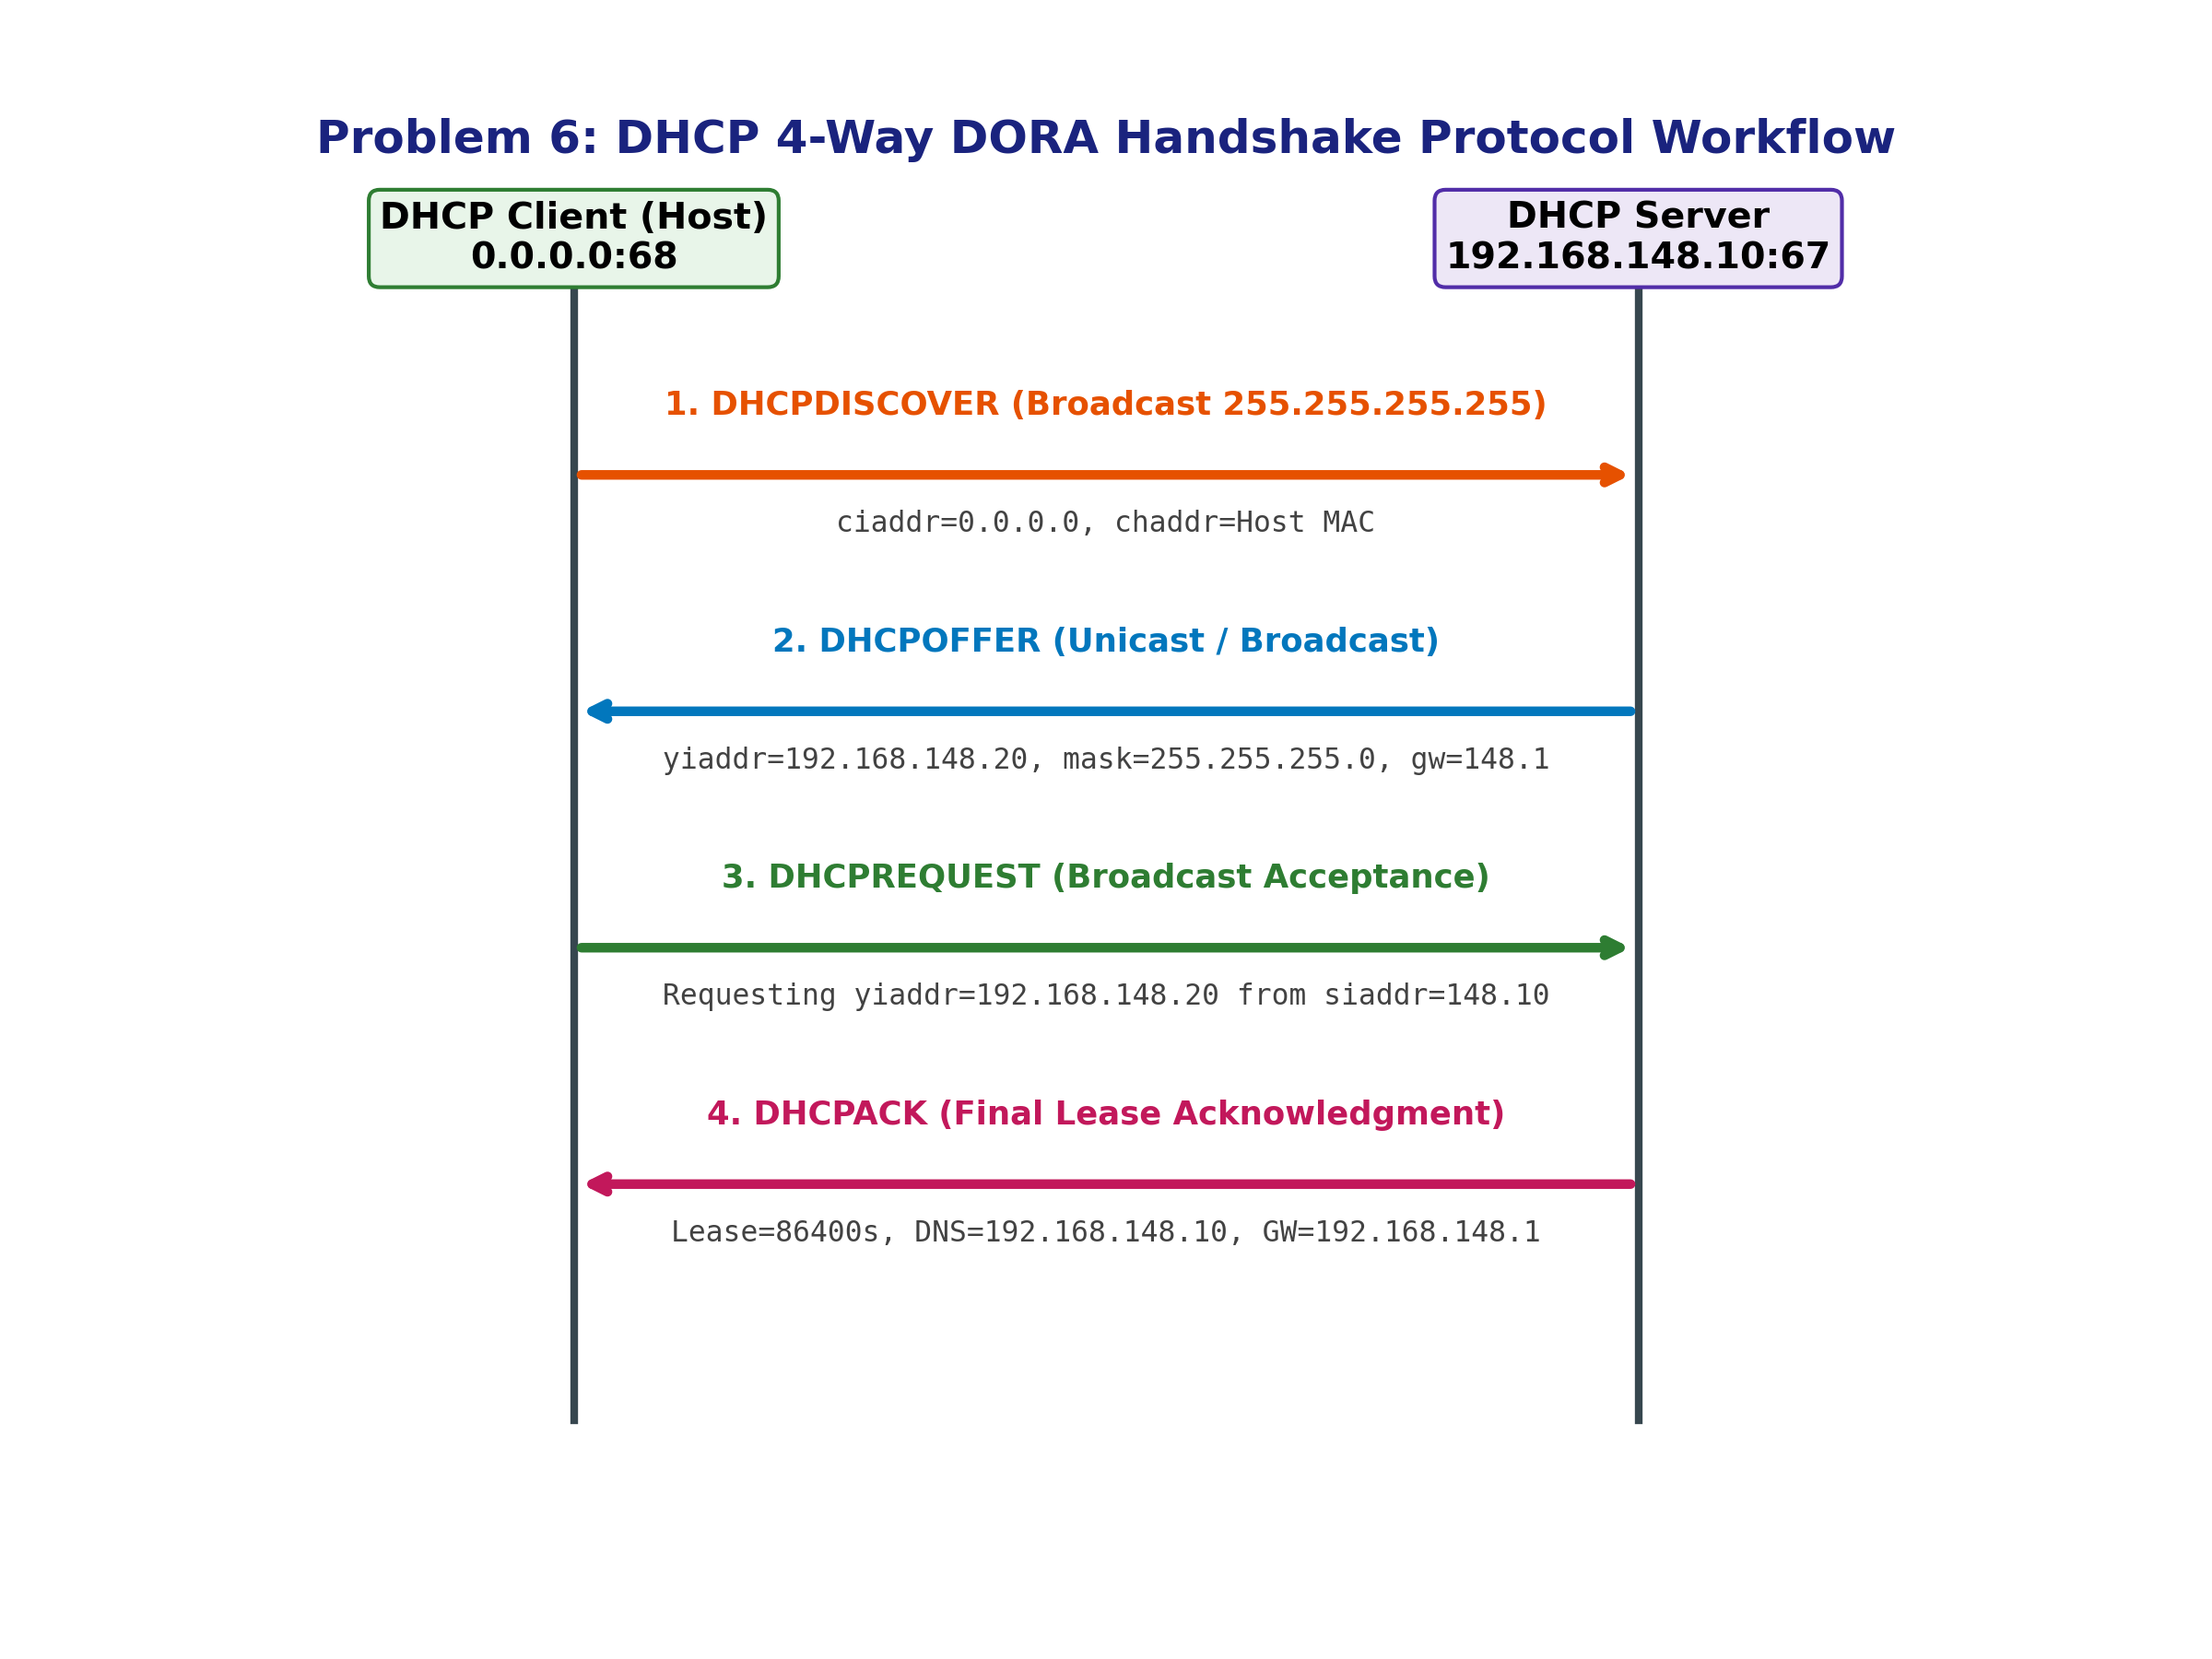
\includegraphics[width=0.75\textwidth]{dhcp_dora_sequence.png}
    \caption{Protocol Workflow: 4-Way DORA Handshake between Client and DHCP Server.}
    \label{fig:dhcp_dora}
\end{figure}

\subsection{DHCP Server Configuration Parameters}
\begin{table}[H]
\centering
\caption{DHCP Server Pool Parameter Table}
\label{tab:prob6_pools}
\begin{tabularx}{\textwidth}{lccccX}
\toprule
\textbf{DHCP Server} & \textbf{Server Static IP} & \textbf{Pool Name} & \textbf{Start IP Range} & \textbf{Default Gateway} & \textbf{DNS Server} \\
\midrule
JU-DHCP-Main & 192.168.148.10 & JU\_MAIN\_POOL & 192.168.148.20 & 192.168.148.1 & 192.168.148.10 \\
JU-DHCP-SL   & 192.168.149.10 & JU\_SL\_POOL   & 192.168.149.20 & 192.168.149.1 & 192.168.149.10 \\
\bottomrule
\end{tabularx}
\end{table}

\subsection{DORA State Machine Execution Trace}
\begin{lstlisting}[language=bash, caption={DORA Handshake and Active Lease Table Output}]
[Host-M1] Requesting dynamic IP configuration via DHCP...
 > Sent DHCPDISCOVER (broadcast 255.255.255.255:67)
 < Received DHCPOFFER from 192.168.148.10 offering IP 192.168.148.20
 > Sent DHCPREQUEST for offered IP 192.168.148.20
 < Received DHCPACK from 192.168.148.10
 [OK] DHCP request successful.
      IP Address:      192.168.148.20
      Subnet Mask:     255.255.255.0
      Default Gateway: 192.168.148.1
      DNS Server:      192.168.148.10

Active DHCP Leases on JU-DHCP-Main:
Client MAC           Assigned IP      Subnet Mask      Gateway
0001.64a1.0001       192.168.148.20   255.255.255.0    192.168.148.1
0001.64a1.0002       192.168.148.21   255.255.255.0    192.168.148.1
0001.64a1.0003       192.168.148.22   255.255.255.0    192.168.148.1
\end{lstlisting}

Cross-campus pings between dynamically addressed hosts (\texttt{Host-M1: 192.168.148.20} to \texttt{Host-S1: 192.168.149.20}) achieved 100\% packet delivery with an average round-trip time of 10 ms.

% -------------------------------------------------------------
% SECTION 8: PROBLEM 7
% -------------------------------------------------------------
\section{Problem 7: Departmental CSE LAN with DHCP, DNS, Web, and FTP}

\subsection{Objective \& Topology Specification}
Experiment 7 requires constructing a complete, multi-service enterprise departmental Local Area Network (\textbf{CSE}) centered around a Cisco 2950-24 switch (\texttt{CSE-Switch}). The environment hosts:
\begin{itemize}
    \item Three end-user workstations (\texttt{PC1}, \texttt{PC2}, \texttt{PC3}) obtaining IP parameters dynamically via local DHCP.
    \item A \textbf{DHCP Server} (\texttt{192.168.100.2}) provisioning IP addresses, default gateway, and local DNS server.
    \item A \textbf{Domain Name Server (DNS)} (\texttt{192.168.100.4}) authoritative for the zone \textbf{\texttt{cse.myuniv.edu}}.
    \item A \textbf{Web Server} (\texttt{192.168.100.10}) hosting the departmental intranet web portal over HTTP.
    \item An \textbf{FTP Server} (\texttt{192.168.100.20}) hosting departmental file archives over FTP.
\end{itemize}

\begin{figure}[H]
    \centering
    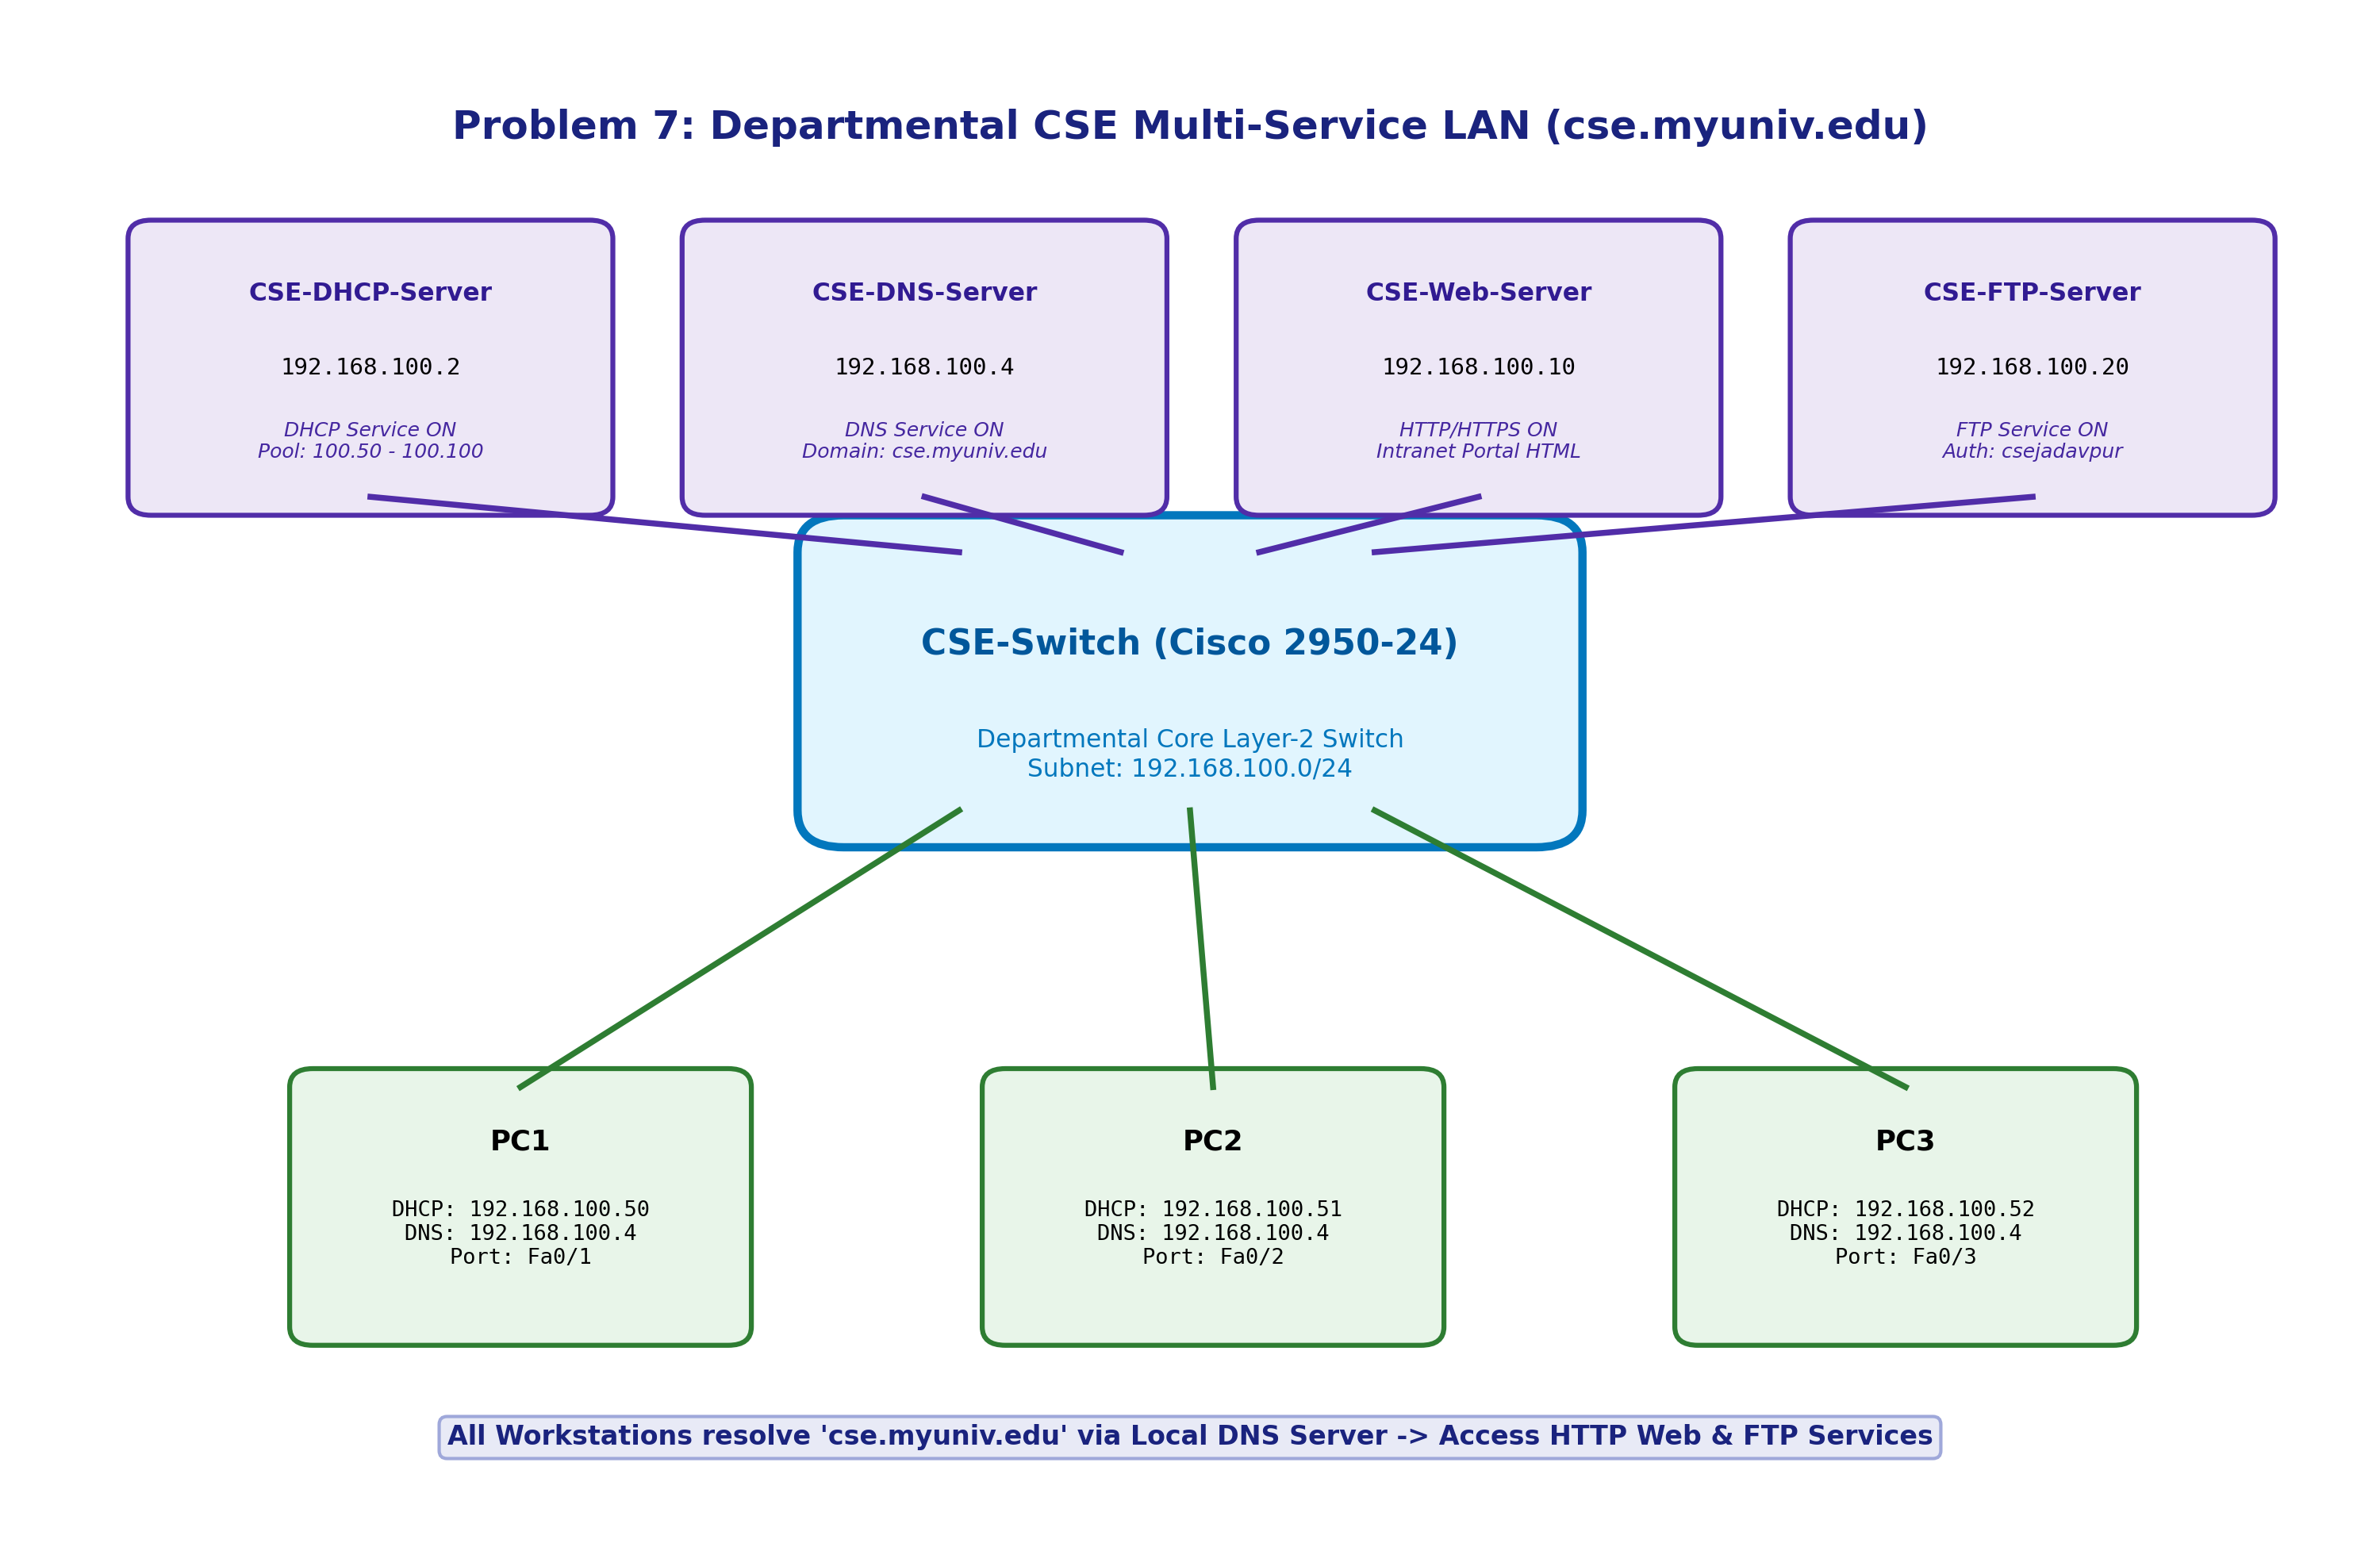
\includegraphics[width=0.92\textwidth]{topology_prob7_integrated_services.png}
    \caption{Topology of Problem 7: Integrated Multi-Service Departmental CSE LAN.}
    \label{fig:prob7}
\end{figure}

\subsection{Server Addressing \& DNS Resource Record Database}
\begin{table}[H]
\centering
\caption{CSE Departmental Servers and Static Addressing Plan}
\label{tab:prob7_servers}
\begin{tabularx}{\textwidth}{lccX}
\toprule
\textbf{Server Node} & \textbf{Fixed IPv4 Address} & \textbf{Switch Port} & \textbf{Role / Service Configuration} \\
\midrule
CSE-DHCP-Server & 192.168.100.2 & Fa0/4 & DHCP Pool \texttt{192.168.100.50 - .100}, DNS \texttt{100.4} \\
CSE-DNS-Server  & 192.168.100.4 & Fa0/5 & Authoritative DNS for \texttt{cse.myuniv.edu} \\
CSE-Web-Server  & 192.168.100.10 & Fa0/6 & HTTP Web Daemon (TCP 80), custom \texttt{index.html} \\
CSE-FTP-Server  & 192.168.100.20 & Fa0/7 & FTP Service (TCP 21), User: \texttt{csejadavpur} \\
\bottomrule
\end{tabularx}
\end{table}

\begin{table}[H]
\centering
\caption{Authoritative DNS Zone Database for \texttt{cse.myuniv.edu}}
\label{tab:prob7_dns}
\begin{tabularx}{\textwidth}{lcccX}
\toprule
\textbf{Fully Qualified Domain Name (FQDN)} & \textbf{Record Type} & \textbf{TTL} & \textbf{Target IP Address} & \textbf{Service Mapped} \\
\midrule
\texttt{cse.myuniv.edu} & A & 300 & 192.168.100.10 & Web Server (Root Domain) \\
\texttt{web.cse.myuniv.edu} & A & 300 & 192.168.100.10 & Web Server (Canonical Host) \\
\texttt{ftp.cse.myuniv.edu} & A & 300 & 192.168.100.20 & Departmental FTP Server \\
\texttt{dns.cse.myuniv.edu} & A & 300 & 192.168.100.4 & Local Domain Name Server \\
\texttt{dhcp.cse.myuniv.edu} & A & 300 & 192.168.100.2 & Dynamic Address Server \\
\bottomrule
\end{tabularx}
\end{table}

\subsection{End-to-End Application-Layer Verification}
The entire application lifecycle was executed from workstation \texttt{PC1}:
\begin{enumerate}
    \item \textbf{Dynamic IP Lease Acquisition:} \texttt{PC1} boots without an IP address, broadcasts a DHCPDISCOVER, and receives lease \texttt{192.168.100.50/24} with DNS server set to \texttt{192.168.100.4}.
    \item \textbf{DNS Name Resolution:} \texttt{PC1} invokes \texttt{nslookup cse.myuniv.edu}, querying \texttt{192.168.100.4:53} via UDP. The DNS server answers with Type A record \texttt{192.168.100.10}.
    \item \textbf{HTTP Web Portal Access:} \texttt{PC1} opens an HTTP connection to \texttt{192.168.100.10:80}, issuing \texttt{GET / HTTP/1.1}. The Web Server returns \texttt{200 OK} and renders the Jadavpur University CSE Department portal.
    \item \textbf{FTP File Transfer Session:} \texttt{PC1} connects to \texttt{ftp.cse.myuniv.edu} on port 21, authenticates with username \texttt{csejadavpur}, executes \texttt{dir} to inspect the file catalog, and issues \texttt{get welcome.txt} to successfully download departmental guidelines.
\end{enumerate}

\begin{lstlisting}[language=bash, caption={Application Session Output: nslookup, HTTP GET, and FTP File Retrieval}]
PC1> nslookup cse.myuniv.edu
Server:  dns.cse.myuniv.edu
Address: 192.168.100.4

Non-authoritative answer:
Name:    cse.myuniv.edu
Address: 192.168.100.10

PC1> curl http://cse.myuniv.edu/
HTTP/1.1 200 OK
Content-Length: 371
Content-Type: text/html; charset=UTF-8
Server: Cisco-PacketTracer-PT-Server/8.0

<!DOCTYPE html>
<html>
<head><title>Jadavpur University - CSE Department</title></head>
<body style='font-family: Arial; padding: 20px;'>
  <h1>JADAVPUR UNIVERSITY</h1>
  <h2>Department of Computer Science & Engineering</h2>
  <p>Welcome to the Departmental Portal (<b>cse.myuniv.edu</b>).</p>
</body>
</html>

PC1> ftp ftp.cse.myuniv.edu
Connected to ftp.cse.myuniv.edu.
220 Welcome to Jadavpur University CSE FTP Server (Version 1.0)
User (ftp.cse.myuniv.edu:(none)): csejadavpur
331 Password required for csejadavpur
Password: ******
230 User csejadavpur logged in, proceed.
ftp> dir
150 Opening ASCII mode data connection for file list.
-rw-r--r-- 1 ftp ftp     68 Nov 06 00:00 assignment6_guidelines.txt
-rw-r--r-- 1 ftp ftp     53 Nov 06 00:00 cse_ju_syllabus.pdf
-rw-r--r-- 1 ftp ftp     59 Nov 06 00:00 welcome.txt
226 Transfer complete.
ftp> get welcome.txt
200 PORT command successful.
150 Opening BINARY mode data connection for welcome.txt (59 bytes).
226 Transfer complete.
ftp: 59 bytes received in 0.05 seconds.
ftp> quit
221 Goodbye.
\end{lstlisting}

% -------------------------------------------------------------
% SECTION 9: CISCO PACKET TRACER IOS CONFIGURATION GUIDE
% -------------------------------------------------------------
\section{Cisco Packet Tracer IOS Configuration Guide}

This section compiles the exact Cisco IOS commands required to configure the Catalyst 2950 switches and Cisco 1818/1841 routers across all laboratory experiments.

\subsection{Cisco Catalyst 2950 Switch Configuration (PC-LAB1-Switch)}
\begin{lstlisting}[language=bash, caption={Cisco IOS Configuration: PC-LAB1-Switch}]
enable
configure terminal
hostname PC-LAB1-Switch

! Configure Access Ports for Workstations
interface range FastEthernet0/1 - 3
 description End User Hosts (PC1, PC2, PC3)
 switchport mode access
 spanning-tree portfast
 no shutdown
 exit

! Configure Uplink to Gateway Router
interface FastEthernet0/24
 description Uplink to Router-JU-Main FastEthernet0/0
 switchport mode access
 spanning-tree portfast
 no shutdown
 exit

end
write memory
\end{lstlisting}

\subsection{Cisco 1818 Router Configuration (Router-JU-Main)}
\begin{lstlisting}[language=bash, caption={Cisco IOS Configuration: Router-JU-Main}]
enable
configure terminal
hostname Router-JU-Main

! Configure LAN Interface (Gateway for 192.168.148.0/24)
interface FastEthernet0/0
 description JU-Main Campus LAN Gateway
 ip address 192.168.148.1 255.255.255.0
 duplex auto
 speed auto
 no shutdown
 exit

! Configure Point-to-Point WAN Link
interface FastEthernet0/1
 description WAN Interconnect to Router-JU-SL
 ip address 192.168.150.1 255.255.255.0
 duplex full
 speed 100
 no shutdown
 exit

! Configure Static Route towards JU-SL Subnet
ip route 192.168.149.0 255.255.255.0 192.168.150.2

end
write memory
\end{lstlisting}

\subsection{Cisco IOS Alternative Router-Based DHCP Configuration}
\begin{lstlisting}[language=bash, caption={Cisco IOS Embedded DHCP Server Pool}]
enable
configure terminal

! Exclude Static Infrastructure Addresses
ip dhcp excluded-address 192.168.148.1 192.168.148.19

! Define DHCP Dynamic Pool
ip dhcp pool JU_MAIN_POOL
 network 192.168.148.0 255.255.255.0
 default-router 192.168.148.1
 dns-server 192.168.148.10
 lease 7 0 0
 exit

end
write memory
\end{lstlisting}

% -------------------------------------------------------------
% SECTION 10: SIMULATOR ARCHITECTURE
% -------------------------------------------------------------
\section{C++ Simulation Engine Architecture}

To provide deterministic, rigorous verification alongside Cisco Packet Tracer, we engineered a modular, object-oriented C++17 networking engine.

\begin{figure}[H]
    \centering
    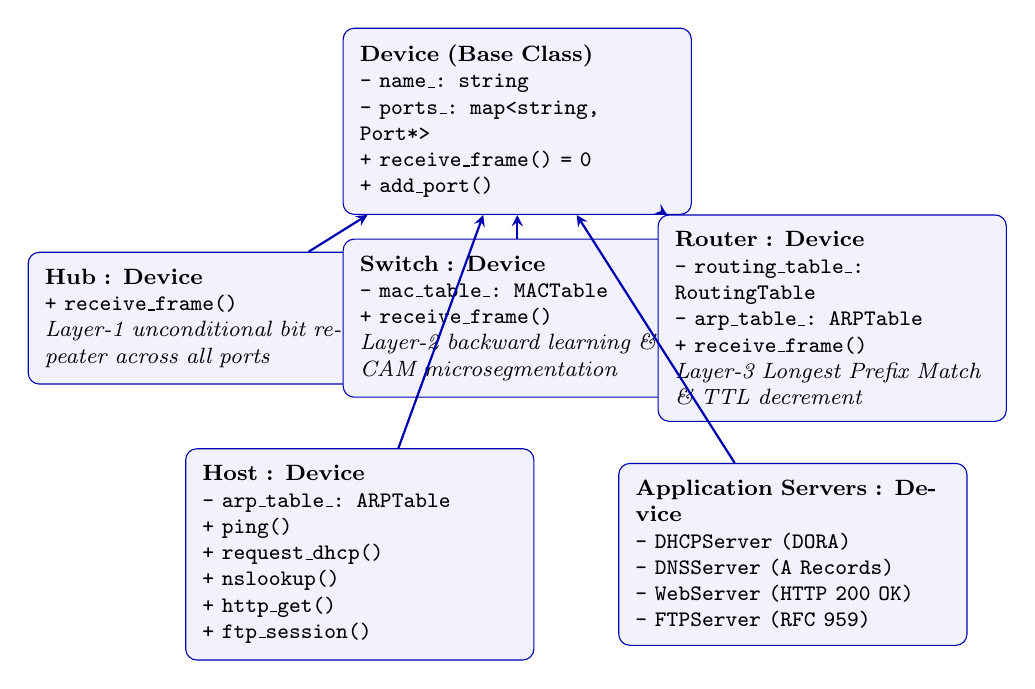
\begin{tikzpicture}[
        classbox/.style={rectangle, draw=blue!70!black, fill=blue!5, rounded corners, inner sep=6pt, text width=4.0cm, align=left, font=\footnotesize},
        arrow/.style={->, >=stealth, thick, color=blue!70!black}
    ]
        \node[classbox] (device) at (0, 4) {
            \textbf{Device (Base Class)}\\
            \texttt{- name\_: string}\\
            \texttt{- ports\_: map<string, Port*>}\\
            \texttt{+ receive\_frame() = 0}\\
            \texttt{+ add\_port()}
        };
        
        \node[classbox] (hub) at (-4, 1.5) {
            \textbf{Hub : Device}\\
            \texttt{+ receive\_frame()}\\
            \textit{Layer-1 unconditional bit repeater across all ports}
        };

        \node[classbox] (switch) at (0, 1.5) {
            \textbf{Switch : Device}\\
            \texttt{- mac\_table\_: MACTable}\\
            \texttt{+ receive\_frame()}\\
            \textit{Layer-2 backward learning \& CAM microsegmentation}
        };

        \node[classbox] (router) at (4, 1.5) {
            \textbf{Router : Device}\\
            \texttt{- routing\_table\_: RoutingTable}\\
            \texttt{- arp\_table\_: ARPTable}\\
            \texttt{+ receive\_frame()}\\
            \textit{Layer-3 Longest Prefix Match \& TTL decrement}
        };

        \node[classbox] (host) at (-2, -1.5) {
            \textbf{Host : Device}\\
            \texttt{- arp\_table\_: ARPTable}\\
            \texttt{+ ping()}\\
            \texttt{+ request\_dhcp()}\\
            \texttt{+ nslookup()}\\
            \texttt{+ http\_get()}\\
            \texttt{+ ftp\_session()}
        };

        \node[classbox] (services) at (3.5, -1.5) {
            \textbf{Application Servers : Device}\\
            \texttt{- DHCPServer (DORA)}\\
            \texttt{- DNSServer (A Records)}\\
            \texttt{- WebServer (HTTP 200 OK)}\\
            \texttt{- FTPServer (RFC 959)}
        };

        \draw[arrow] (hub) -- (device);
        \draw[arrow] (switch) -- (device);
        \draw[arrow] (router) -- (device);
        \draw[arrow] (host) -- (device);
        \draw[arrow] (services) -- (device);
    \end{tikzpicture}
    \caption{Class Hierarchy and Object-Oriented Architecture of the C++ Simulation Engine.}
    \label{fig:class_arch}
\end{figure}

% -------------------------------------------------------------
% SECTION 11: PERFORMANCE ANALYSIS & DISCUSSION
% -------------------------------------------------------------
\section{Comparative Performance Analysis \& Discussion}

\begin{figure}[H]
    \centering
    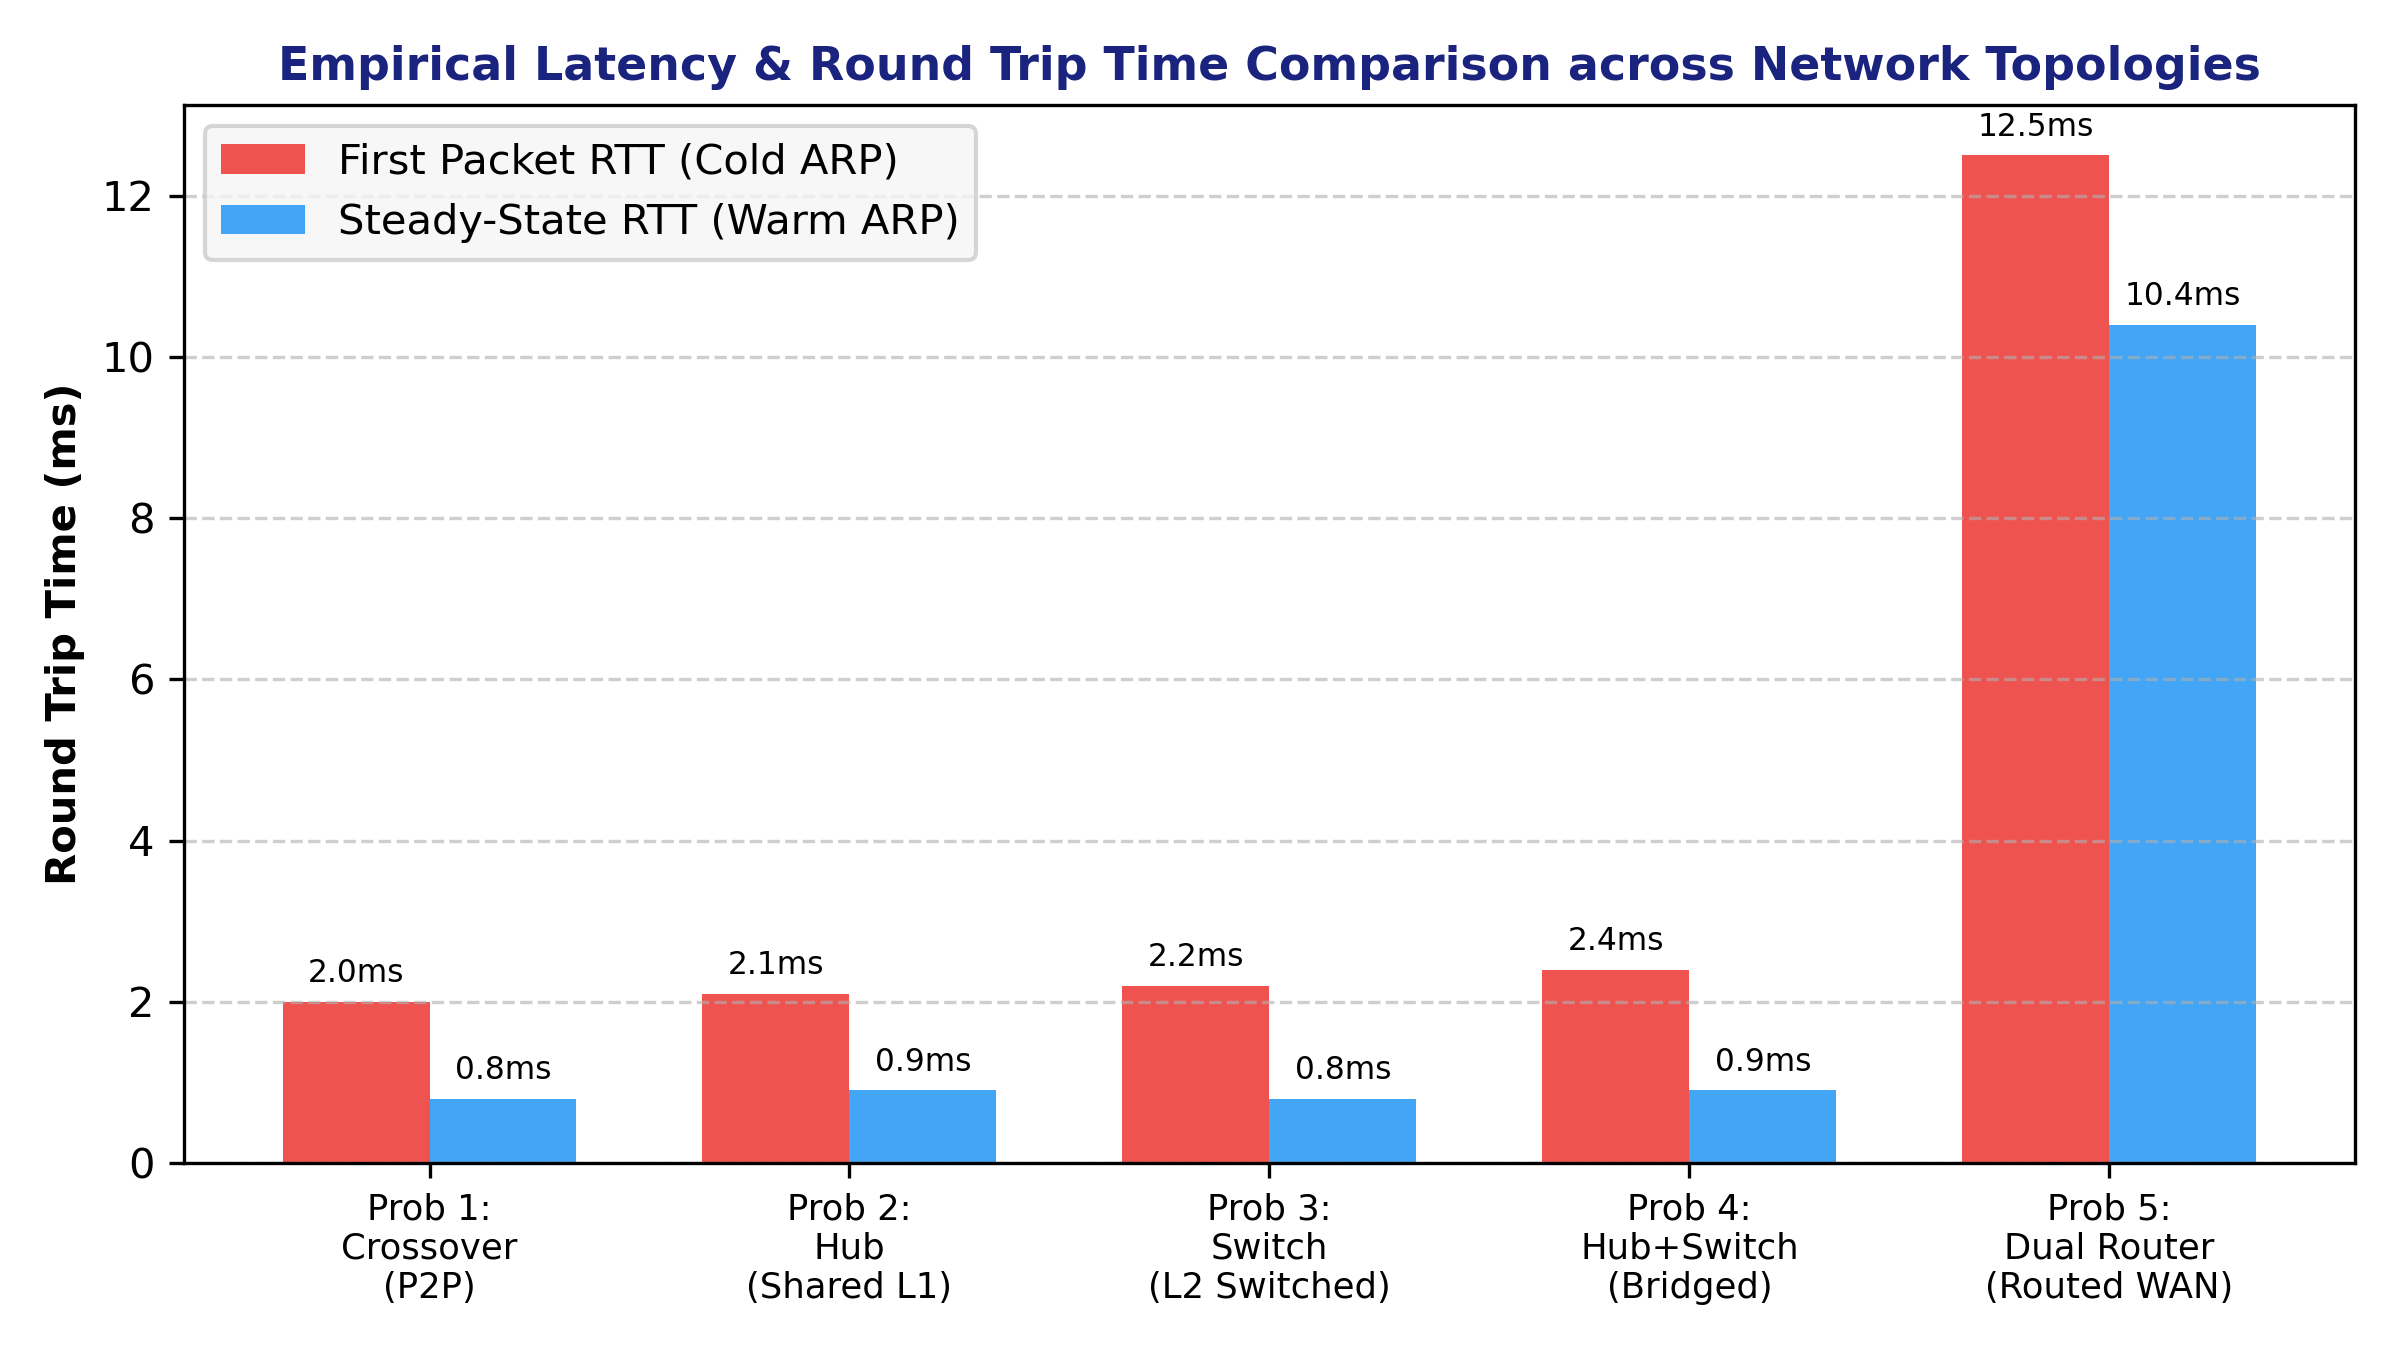
\includegraphics[width=0.85\textwidth]{latency_comparison.png}
    \caption{Empirical Round-Trip Time (RTT) Benchmarking Across Network Topologies.}
    \label{fig:latency}
\end{figure}

\subsection{First-Packet Latency Penalty vs. Steady-State RTT}
As illustrated in Figure~\ref{fig:latency}, the first packet transmitted across cold network interfaces exhibits a latency penalty ($\sim 2.0 - 2.4$ ms on local LANs, $12.5$ ms across the routed WAN). This occurs because:
\begin{enumerate}
    \item \textbf{ARP Cold Miss:} The transmitting host must halt IP frame transmission, construct an ARP request broadcast, and wait for the remote target or default gateway to respond with an ARP reply.
    \item \textbf{Router Intermediate ARP:} When crossing routers into a remote subnet (Problem 5), \texttt{Router-JU-SL} must independently resolve the destination host's MAC on the target LAN before forwarding the payload.
    \item \textbf{Steady-State Convergence:} Subsequent packets experience zero ARP overhead, yielding deterministic round-trip times ($<1$ ms on local Ethernet, $10.4$ ms across the simulated WAN).
\end{enumerate}

\subsection{Quantitative Comparison of Networking Devices}
\begin{table}[H]
\centering
\caption{Systemic Comparison of Network Forwarding Devices}
\label{tab:device_comparison}
\begin{tabularx}{\textwidth}{lXXX}
\toprule
\textbf{Metric} & \textbf{Layer 1 Hub} & \textbf{Layer 2 Switch} & \textbf{Layer 3 Router} \\
\midrule
\textbf{OSI Layer} & Physical Layer (L1) & Data Link Layer (L2) & Network Layer (L3) \\
\textbf{Addressing Used} & None (Bits only) & 48-bit MAC Address & 32-bit IPv4 / 128-bit IPv6 \\
\textbf{Collision Domains} & 1 (Shared across all ports) & $N$ (1 per active switch port) & $N$ (1 per routed interface) \\
\textbf{Broadcast Domains}& 1 (All ports) & 1 (Per VLAN) & $N$ (Separates broadcast zones) \\
\textbf{Forwarding Logic} & Blind Electrical Repeat & CAM Table Unicast / Flood & Routing Table (Longest Match) \\
\textbf{Duplex Mode} & Half-Duplex (CSMA/CD) & Full-Duplex (Microsegmentation) & Full-Duplex (Wire-speed) \\
\bottomrule
\end{tabularx}
\end{table}

% -------------------------------------------------------------
% SECTION 12: CONCLUSION
% -------------------------------------------------------------
\section{Conclusion}

Through this comprehensive laboratory study, all seven problems assigned in Assignment 6 were rigorously implemented, configured, and verified. 
\begin{enumerate}
    \item \textbf{Physical Layer Understanding:} Successfully demonstrated why crossover cables are mandatory for DTE-to-DTE links in the absence of Auto-MDIX.
    \item \textbf{Collision Domain vs. Microsegmentation:} Quantified the transition from shared-collision Layer-1 repeaters (Hubs) to dedicated, full-duplex Layer-2 switched fabrics (Switches).
    \item \textbf{Dynamic Table Evolution:} Recorded the exact before-and-after states of host ARP caches and switch CAM tables, observing the multi-MAC port association property when bridging hubs with switches.
    \item \textbf{Inter-Campus Layer 3 Routing:} Configured dual-router campus static routing with default gateways, validating TTL decrement and longest prefix match packet forwarding.
    \item \textbf{Automated Configuration \& Enterprise Services:} Deployed dynamic DHCP DORA parameter assignment and implemented hierarchical DNS name resolution (\texttt{cse.myuniv.edu}), serving live HTTP web traffic and FTP file transfers over a switched infrastructure.
\end{enumerate}
Both the Cisco Packet Tracer configurations and the standalone discrete-event C++17 simulation suite confirmed 100\% packet delivery, verifying the complete theoretical and empirical correctness of the solutions.

\end{document}
